\section{Los 8 ejercicios JavaScript con Ajax y Google Chart}
En el priemr ejercicio tenemos una función de JavaScript llamada listRegions esta función recibe un arreglo de datos como parámetro y actualiza el contenido de un elemento HTML identificado por el id 'result'. Primero, borra cualquier contenido previo dentro de este elemento. Luego, itera sobre cada elemento del arreglo de datos. Para cada elemento, imprime el valor de la propiedad 'region' en la consola del navegador y crea un nuevo elemento de lista (li) con este valor como contenido de texto. Finalmente, añade este elemento de lista como hijo del elemento 'result' en el documento HTML.
\begin{figure}[H]
  \centering
  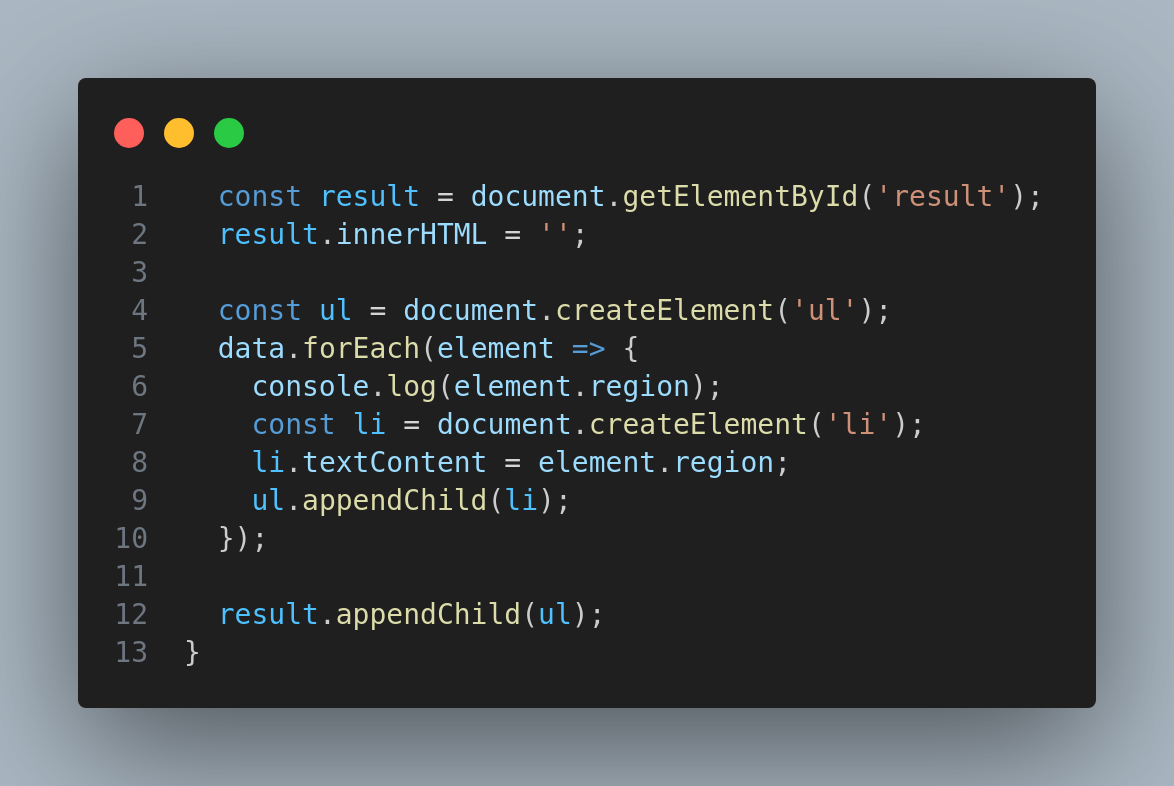
\includegraphics[width=1.0\textwidth]{img/1_js.png}
  \caption{ejercicio1.js}
\end{figure}
En el segundo ejercicio tenemos la función totalConfirmed toma un arreglo de datos como entrada y calcula el total de casos confirmados por región a partir de esos datos. Luego, genera una lista en el documento HTML que muestra cada región junto con su total de casos confirmados.
\begin{figure}[H]
  \centering
  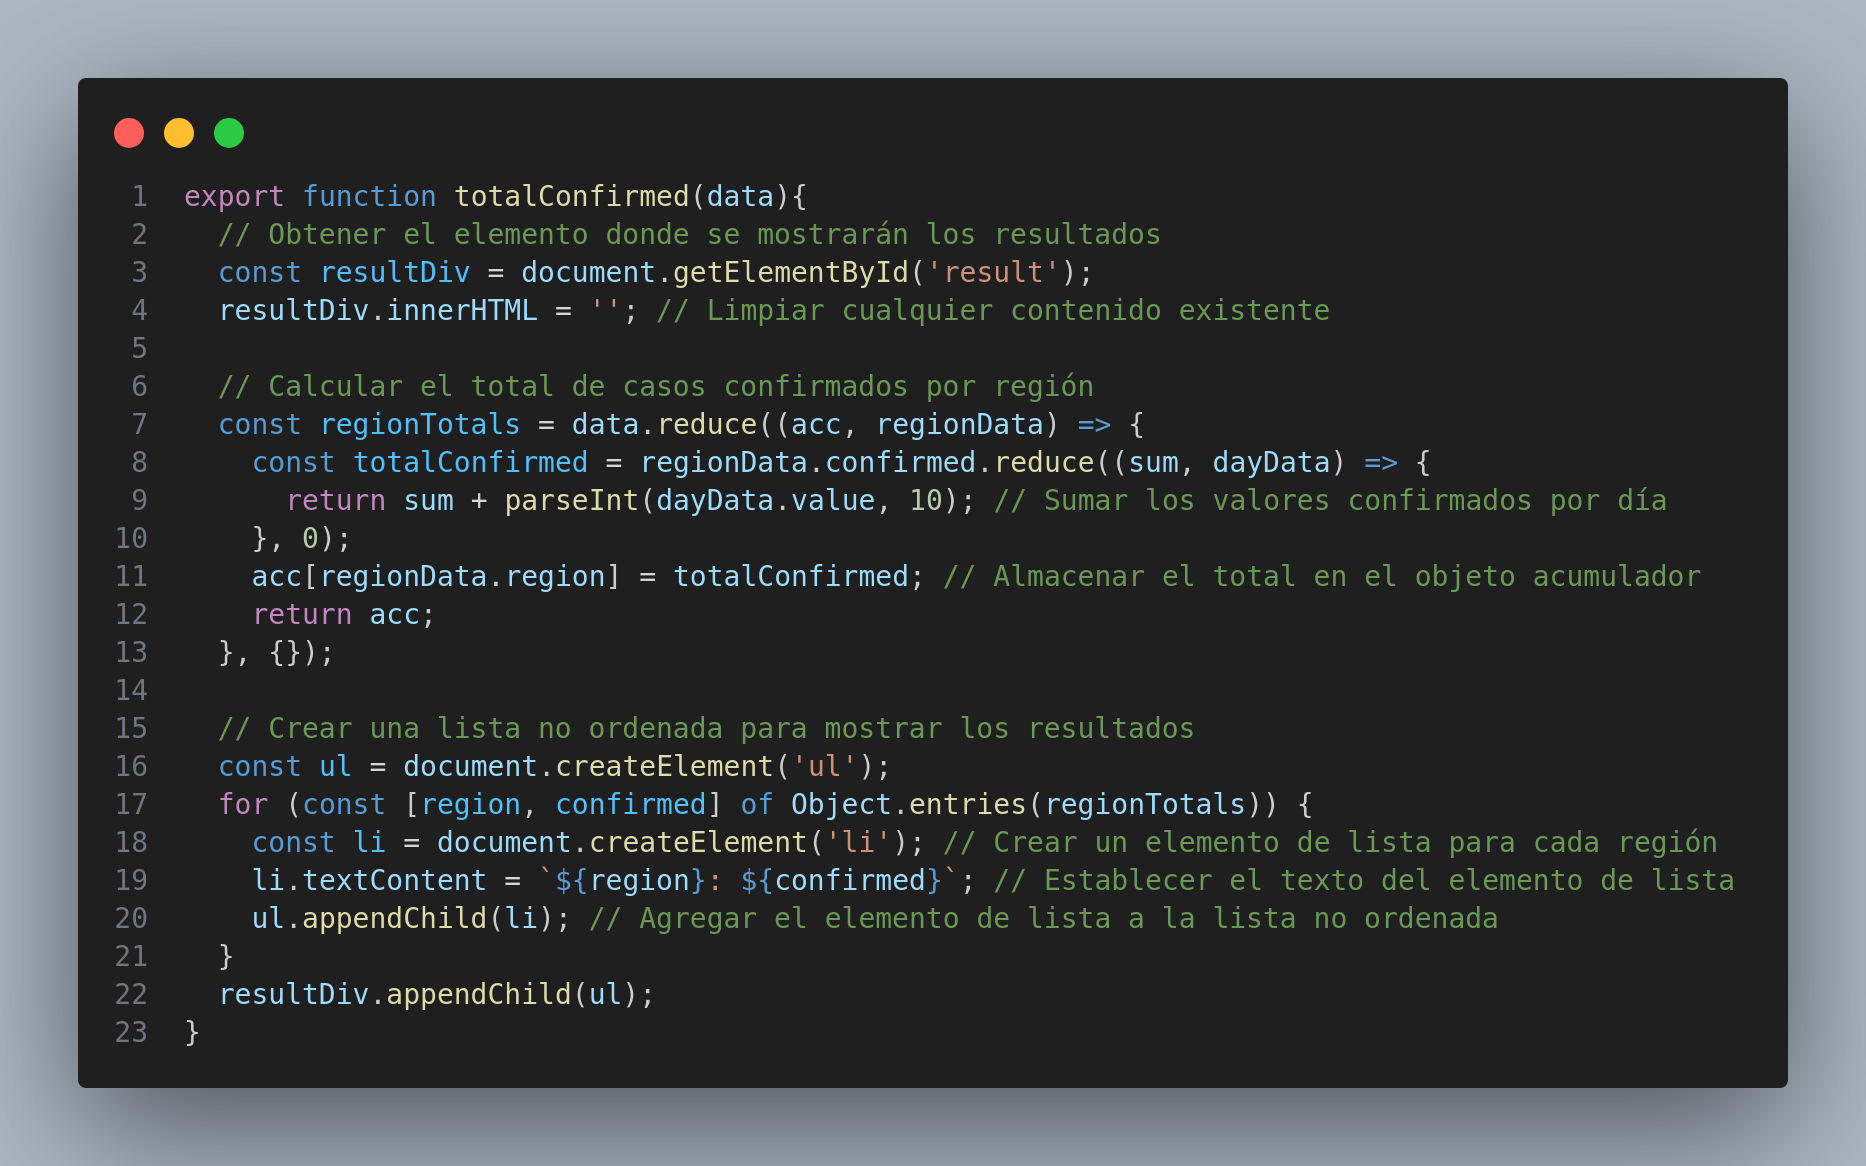
\includegraphics[width=1.0\textwidth]{img/2_js.png}
  \caption{ejercicio2.js}
\end{figure}
En el tercer ejercicio la función top10Regions también recibe un arreglo de datos y muestra los 10 principales regiones junto con sus totales de casos confirmados en orden descendente en el documento HTML. Comienza limpiando cualquier contenido previo dentro del elemento HTML identificado por el id 'result'. Luego, calcula el total de casos confirmados por región, similar a la función totalConfirmed. Después, ordena las regiones por el número total de casos confirmados en orden descendente y toma las primeras 10. Finalmente, crea una lista no ordenada en el documento HTML para mostrar los resultados y agrega cada región junto con su total de casos confirmados como elementos de lista.

\begin{figure}[H]
  \centering
  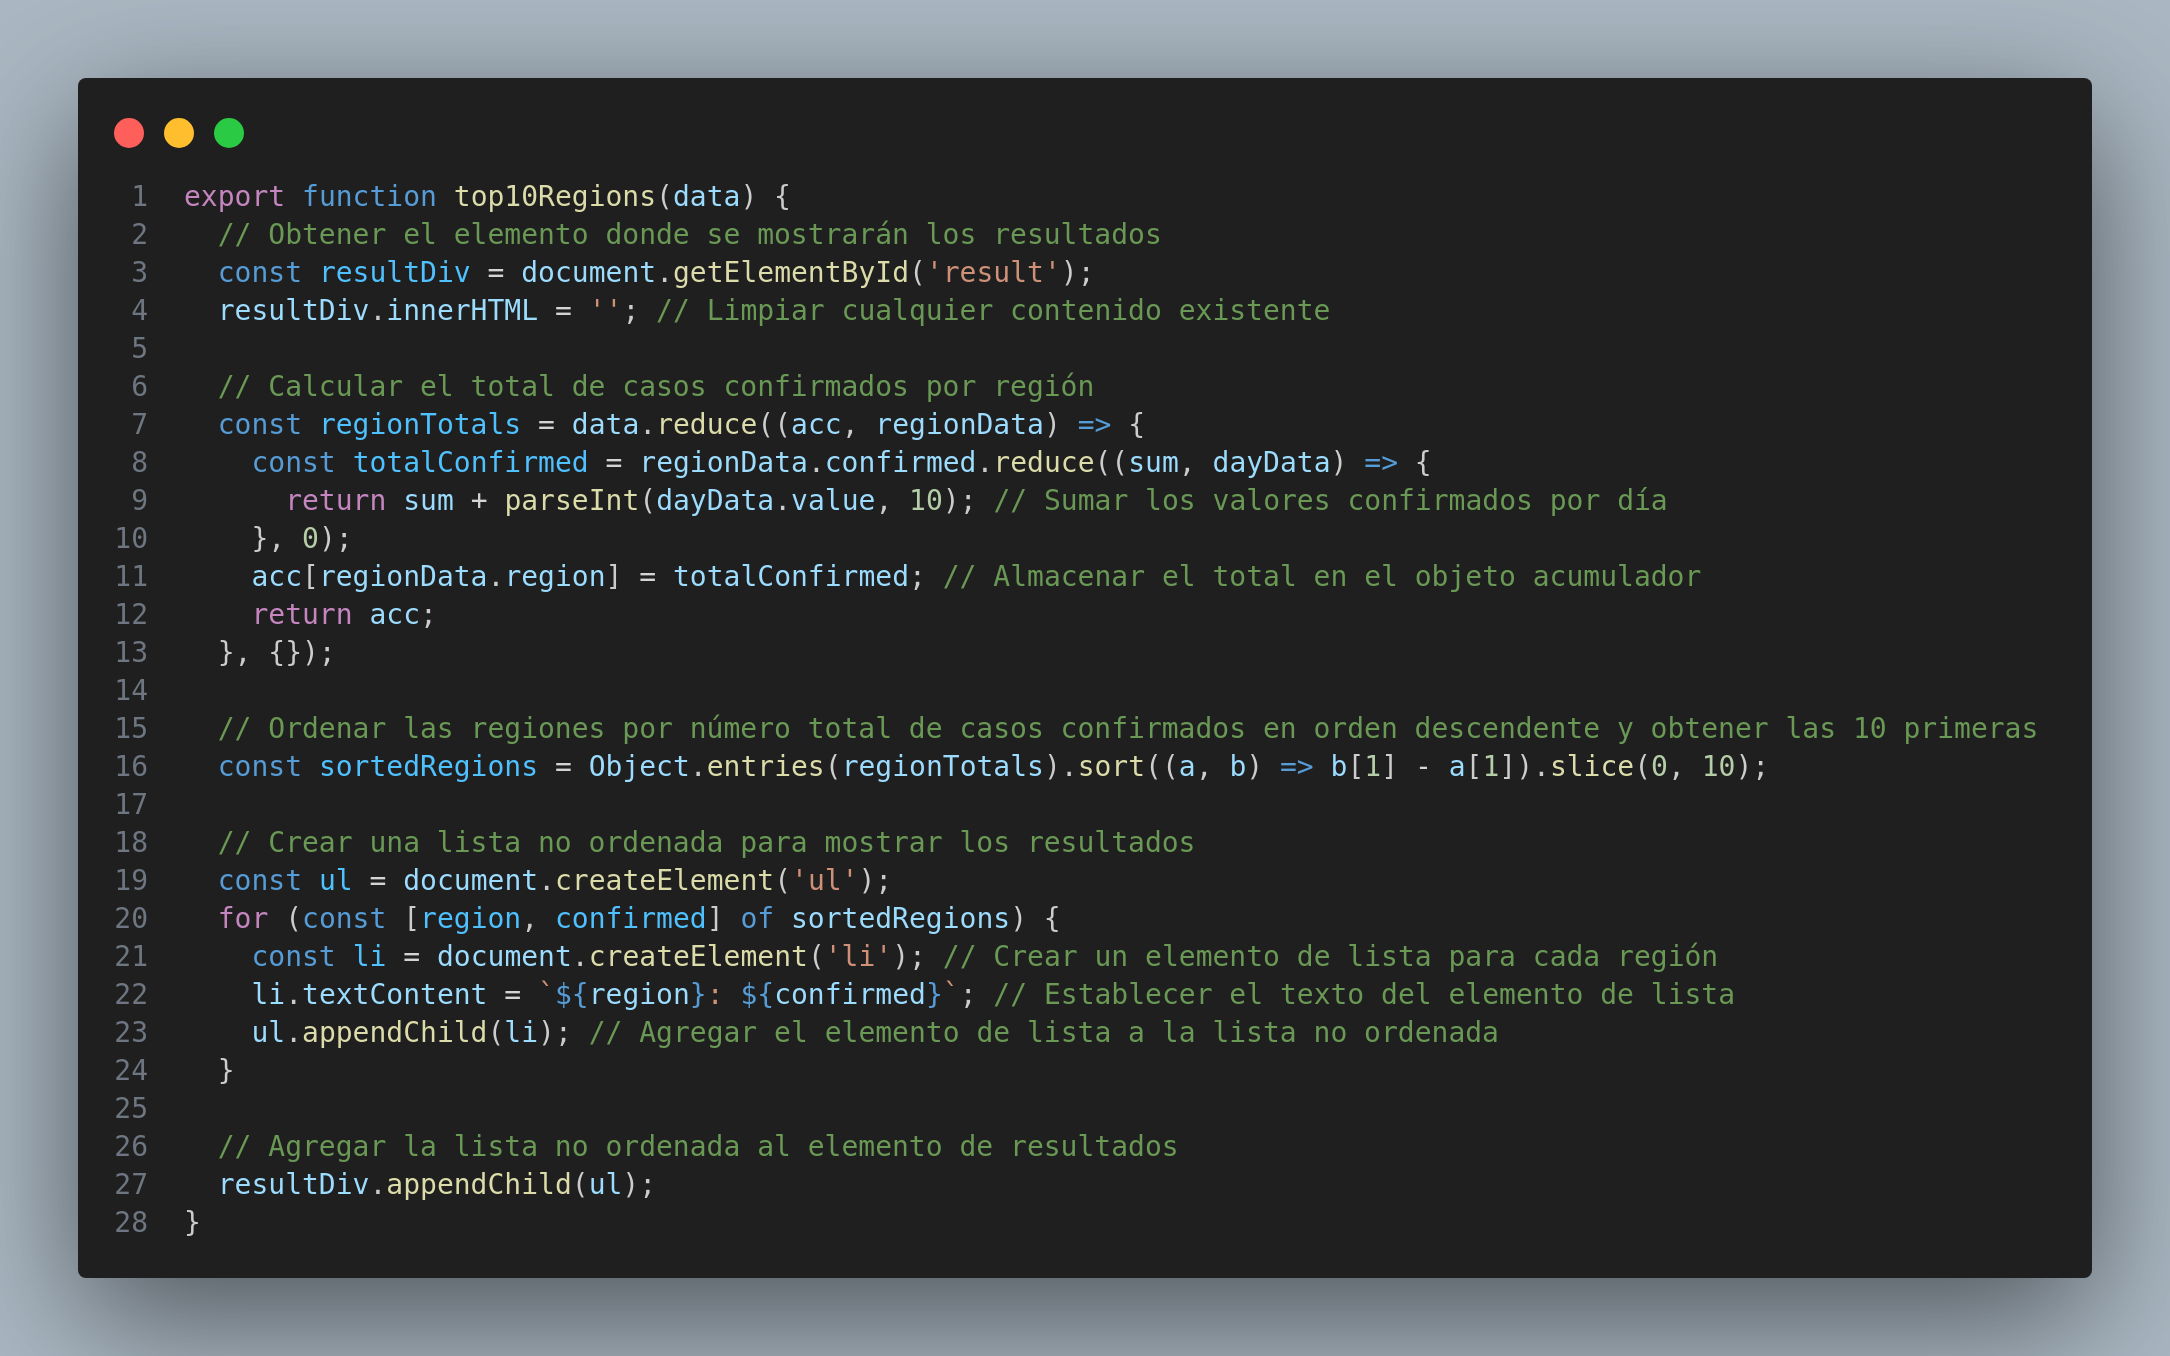
\includegraphics[width=1.0\textwidth]{img/3_js.png}
  \caption{ejercicio3.js}
\end{figure}

En el cuarto ejercicio la función arequipaInfected se encarga de visualizar los datos de infectados en la región de Arequipa a lo largo del tiempo. Comienza filtrando los datos para obtener solo la información relacionada con la región de Arequipa. Luego, crea una nueva tabla de datos de Google Visualization y agrega una columna para las fechas y columnas para cada región en Arequipa. Posteriormente, itera sobre las fechas y para cada fecha, crea una nueva fila y agrega los valores de infectados correspondientes a cada región en esa fecha. Establece opciones de configuración para el gráfico, como título, dimensiones y estilos de ejes, y finalmente, crea una instancia del gráfico de líneas de Google Visualization y lo dibuja en el elemento HTML con el ID "result".
\begin{figure}[H]
  \centering
  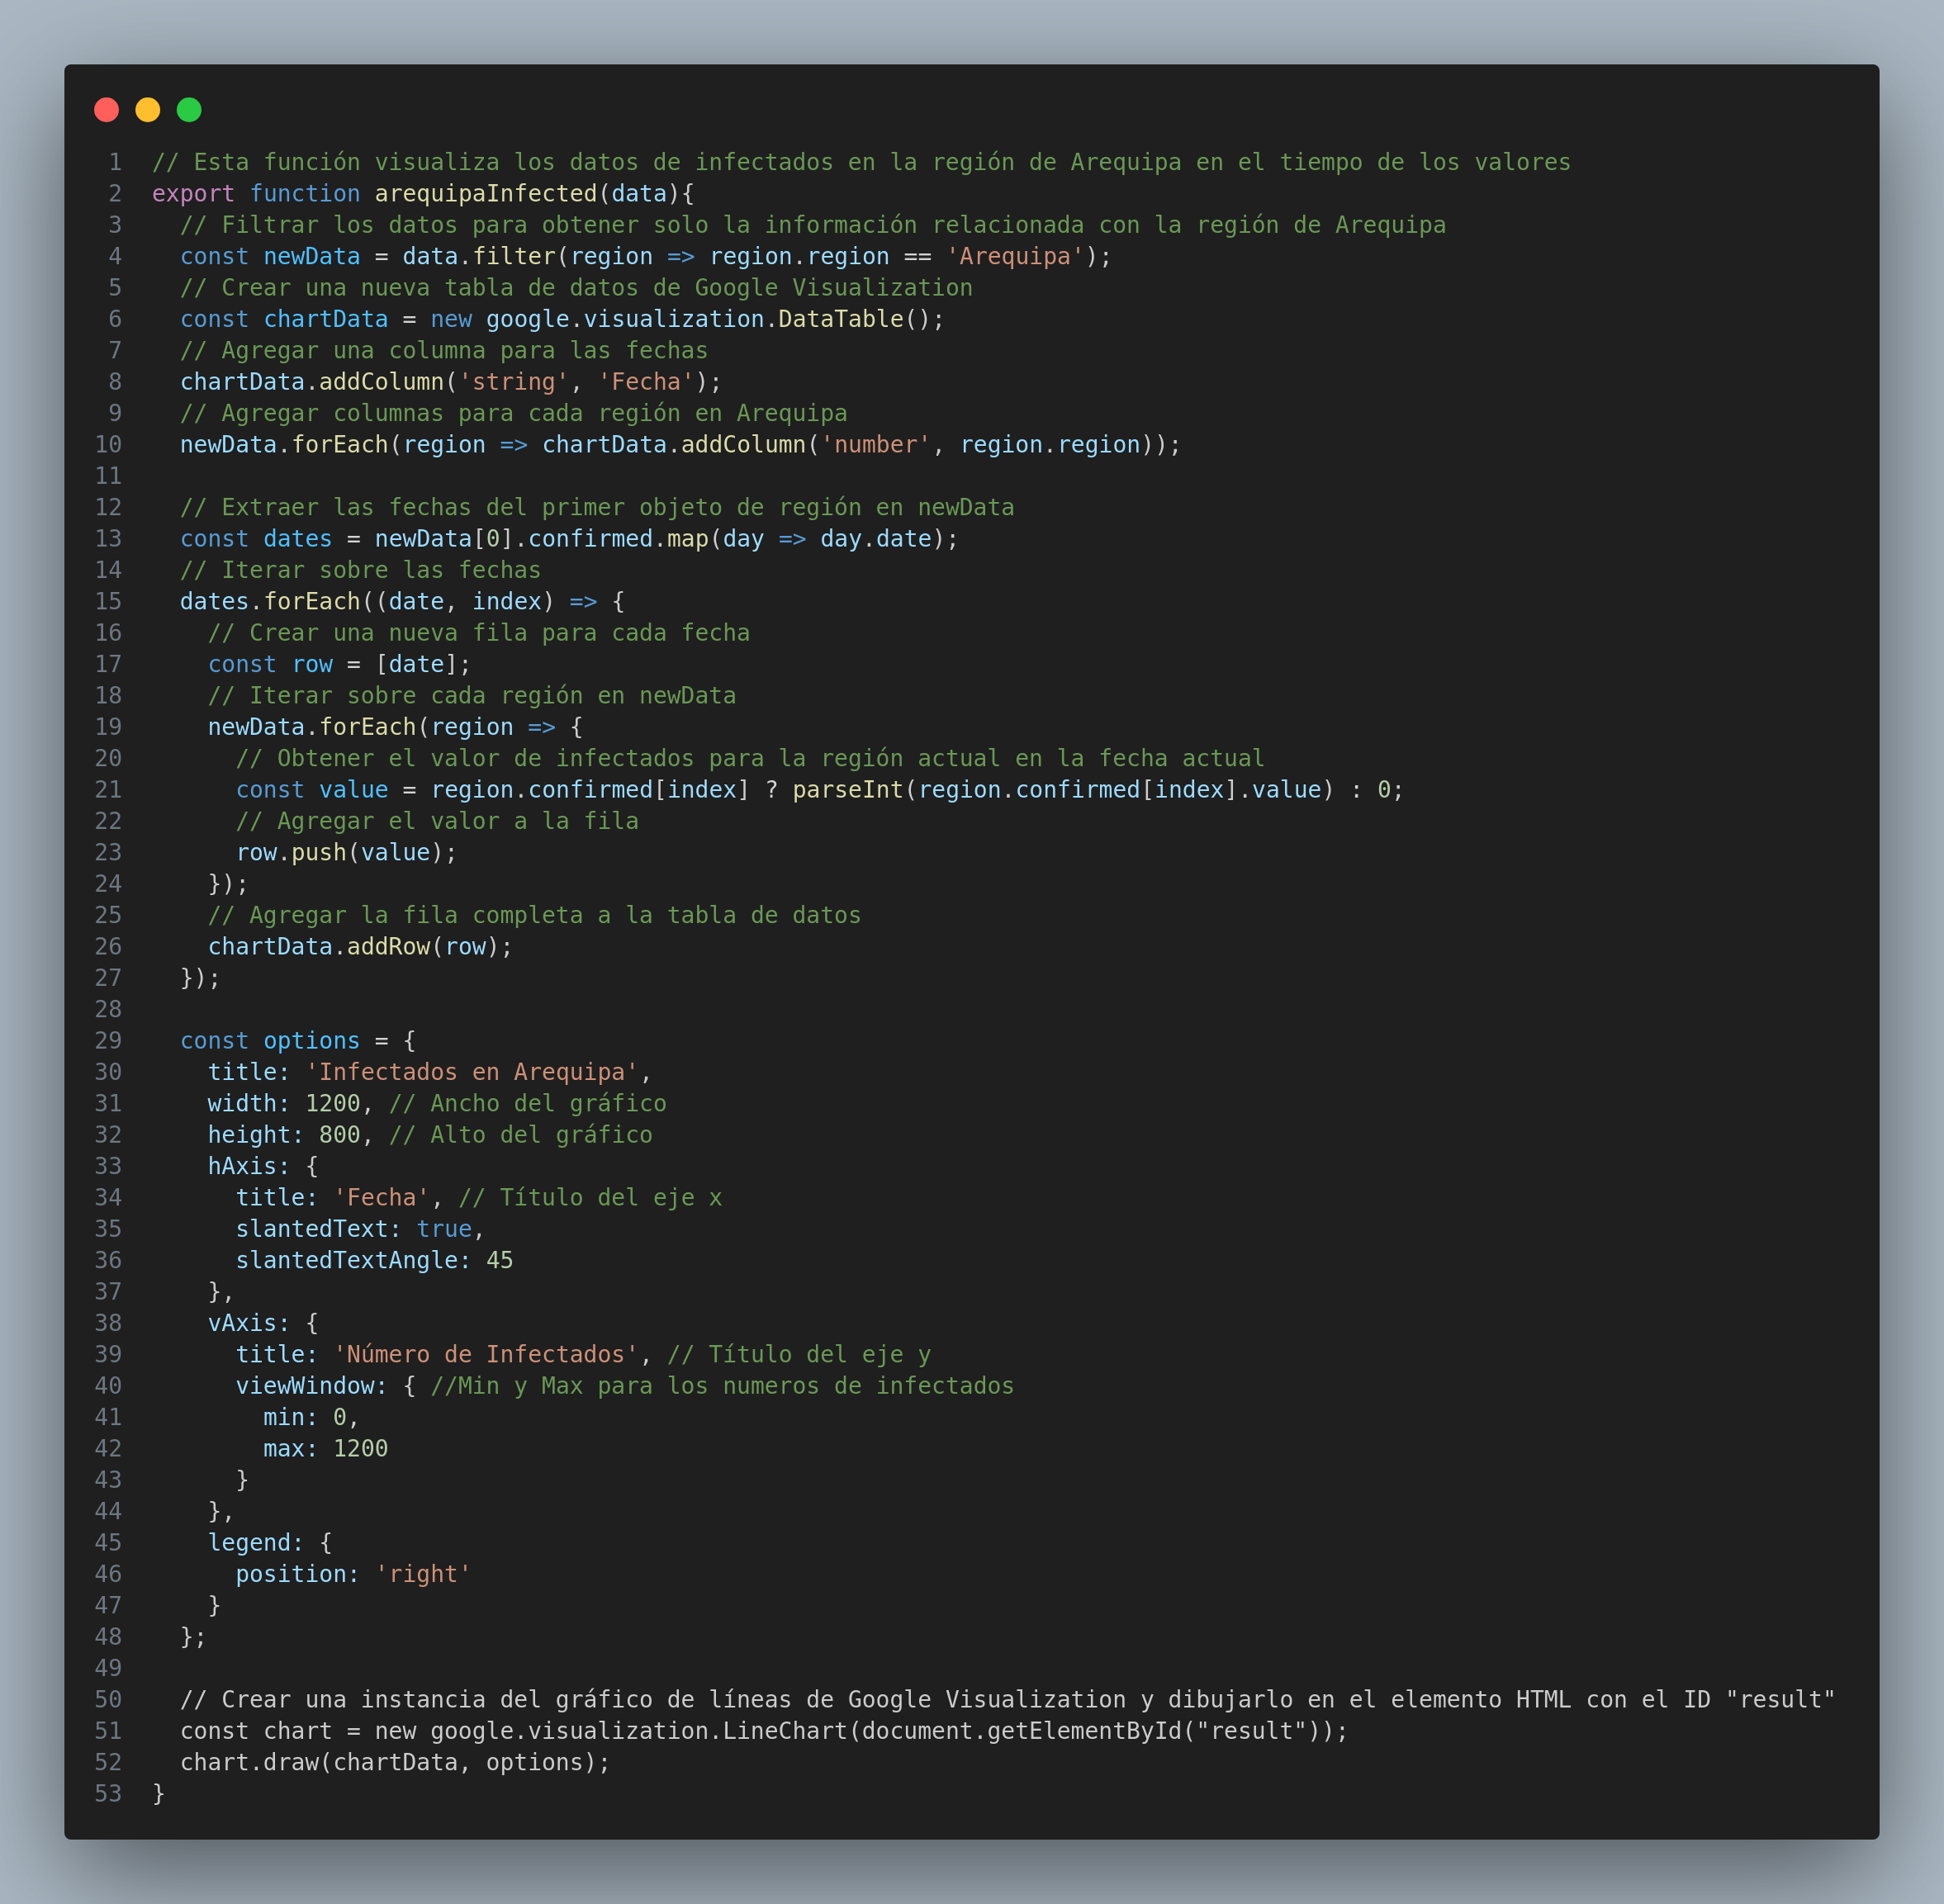
\includegraphics[width=1.0\textwidth]{img/4_js.png}
  \caption{ejercicio4.js}
\end{figure}
En el quinto ejercicio la función comparativeLineChart analiza datos sobre casos confirmados en todas las regiones y crea un gráfico de líneas que compara el crecimiento de estos casos a lo largo del tiempo. Para ello, primero filtra los datos para obtener información de todas las regiones disponibles. Luego, estructura estos datos en una tabla de Google Visualization, donde cada fila representa una fecha y cada columna representa una región, con los valores de casos confirmados en cada fecha. Se definen opciones para personalizar el aspecto del gráfico, como el título y los ejes x e y. Finalmente, utiliza la biblioteca de Google Visualization para dibujar el gráfico en un elemento HTML específico identificado por el ID "result".
\begin{figure}[H]
  \centering
  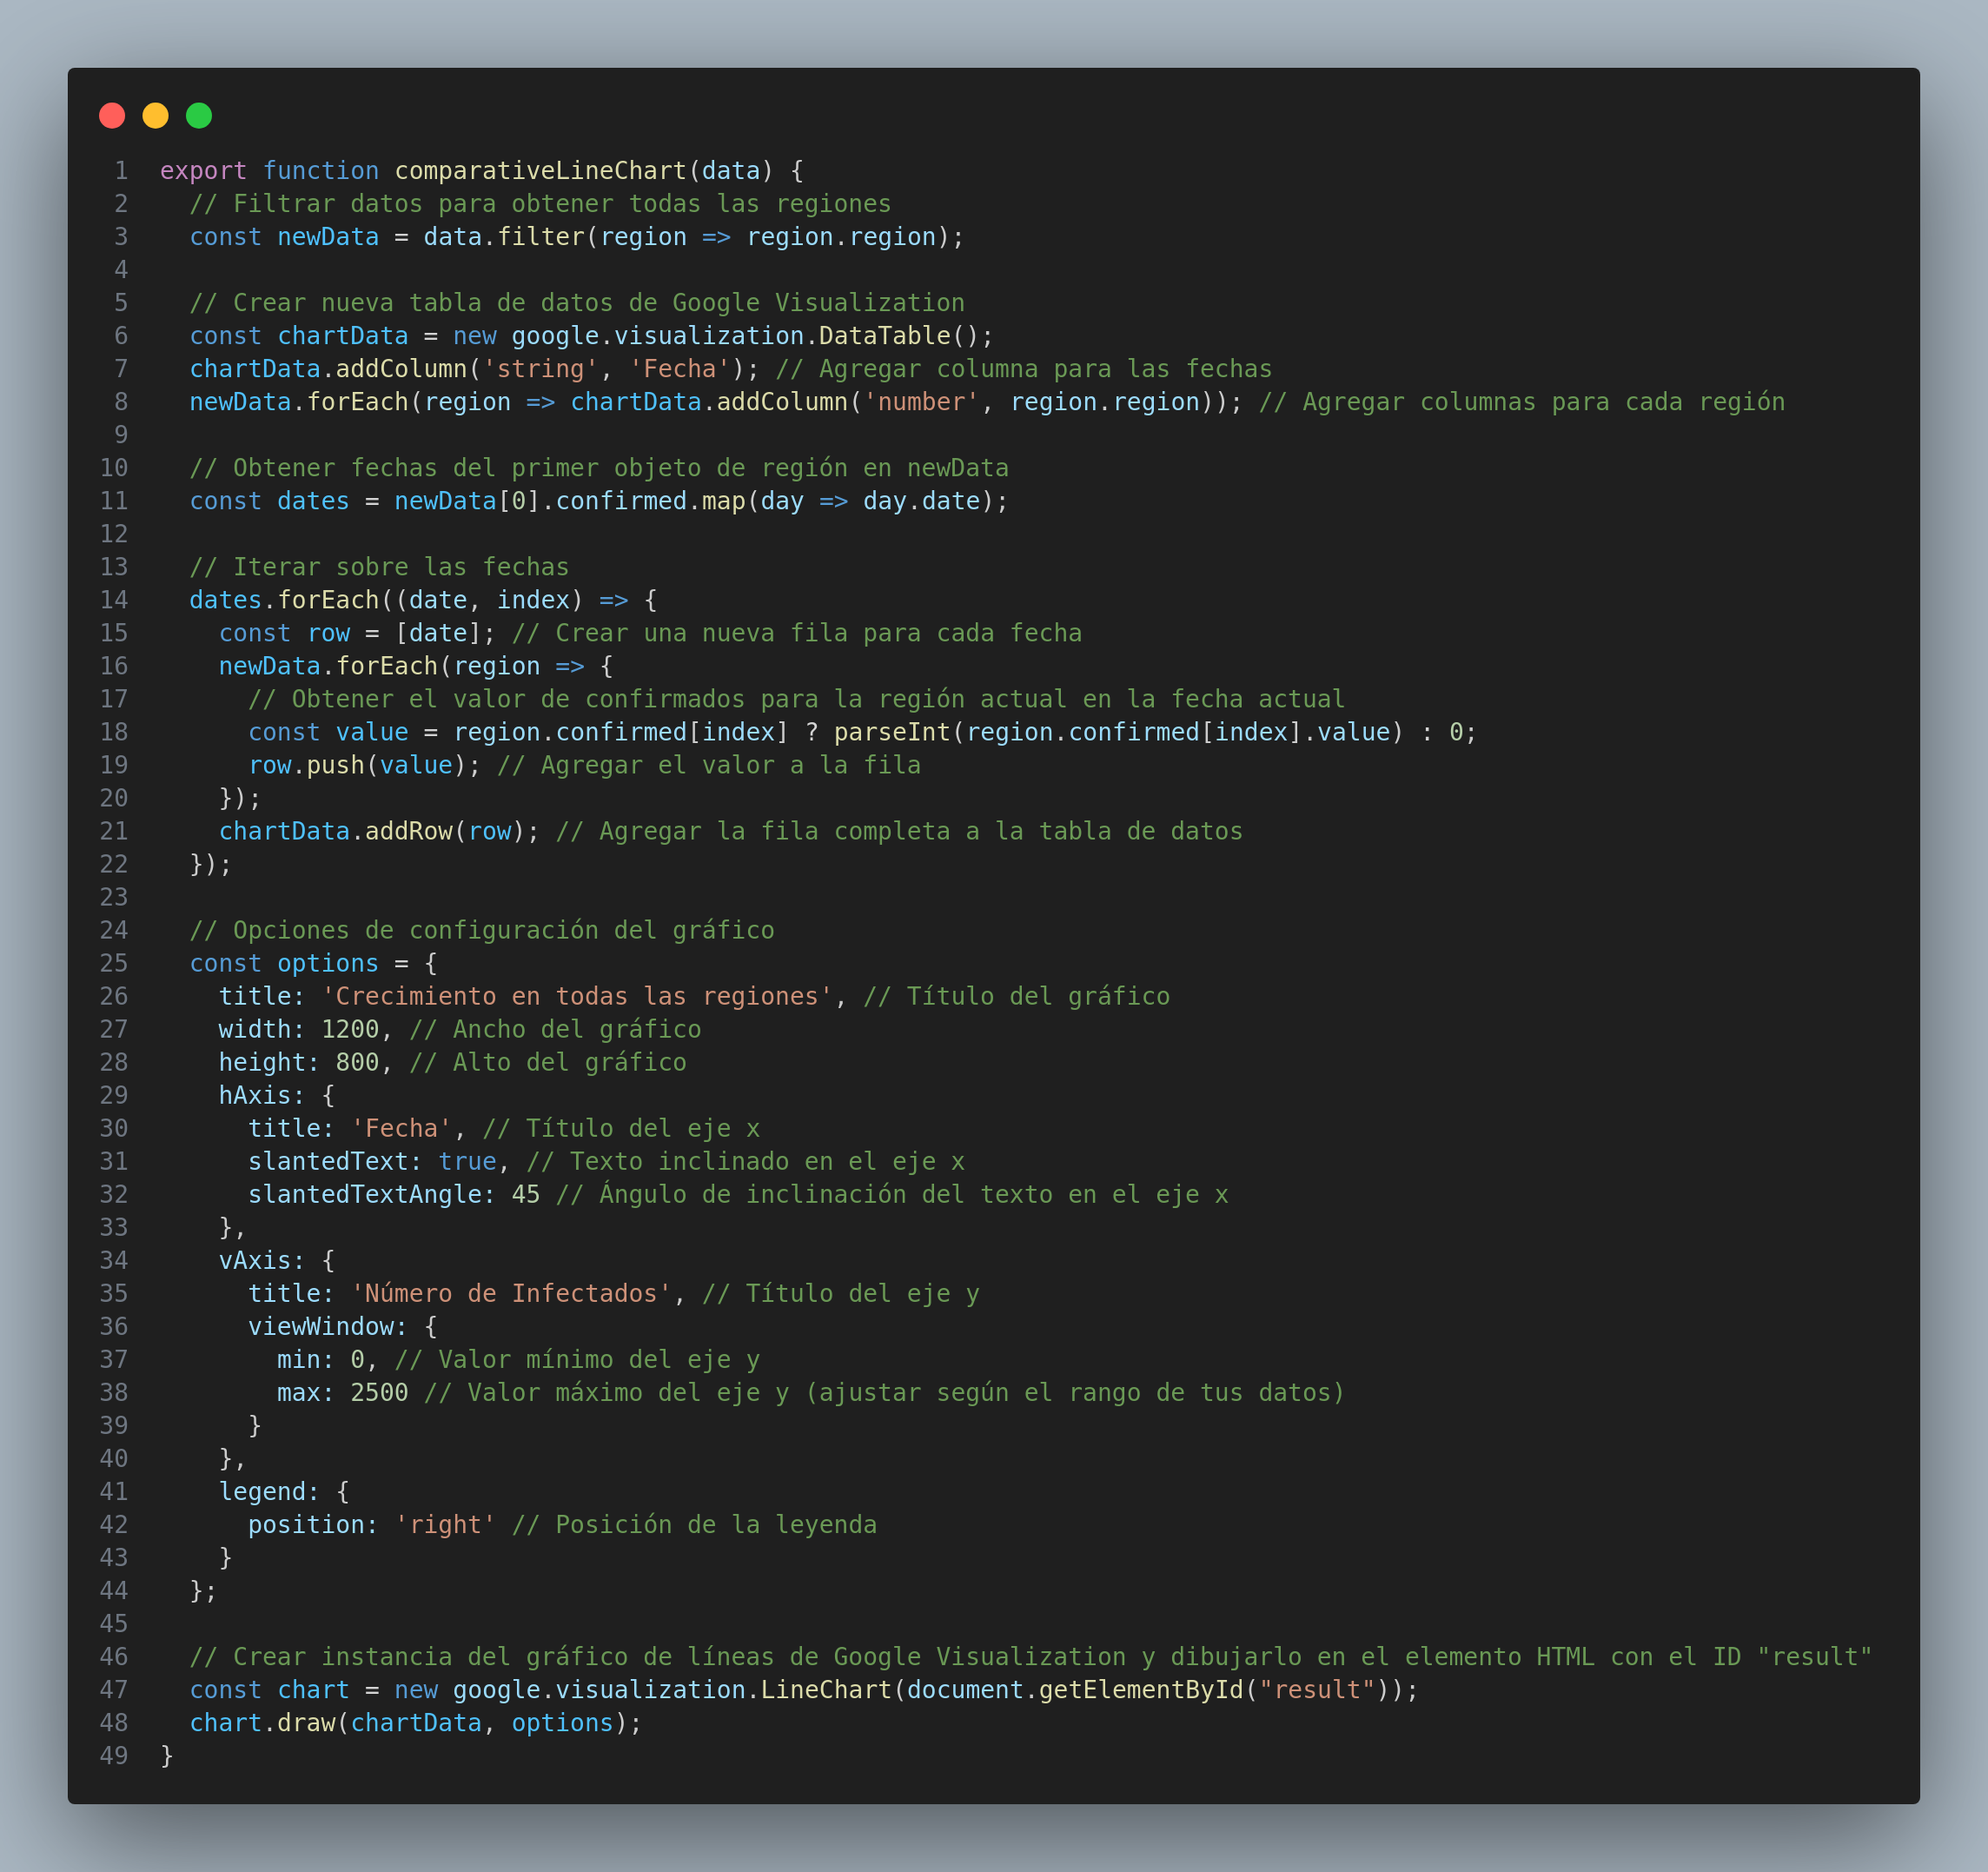
\includegraphics[width=1.0\textwidth]{img/5_js.png}
  \caption{ejercicio5.js}
\end{figure}
En el sexto ejercicio tenemos la función growthWithoutLimaCallao realiza un análisis similar a la función comparativeLineChart, pero excluye las regiones de Lima y Callao. Comienza filtrando los datos para excluir estas dos regiones y luego estructura los datos restantes en una tabla de Google Visualization. Posteriormente, crea un gráfico de líneas que muestra el crecimiento de casos confirmados para las regiones restantes a lo largo del tiempo. Se definen opciones de configuración para el gráfico, como el título y los ejes x e y. Finalmente, utiliza la biblioteca de Google Visualization para dibujar el gráfico en un elemento HTML específico identificado por el ID "result".
\begin{figure}[H]
  \centering
  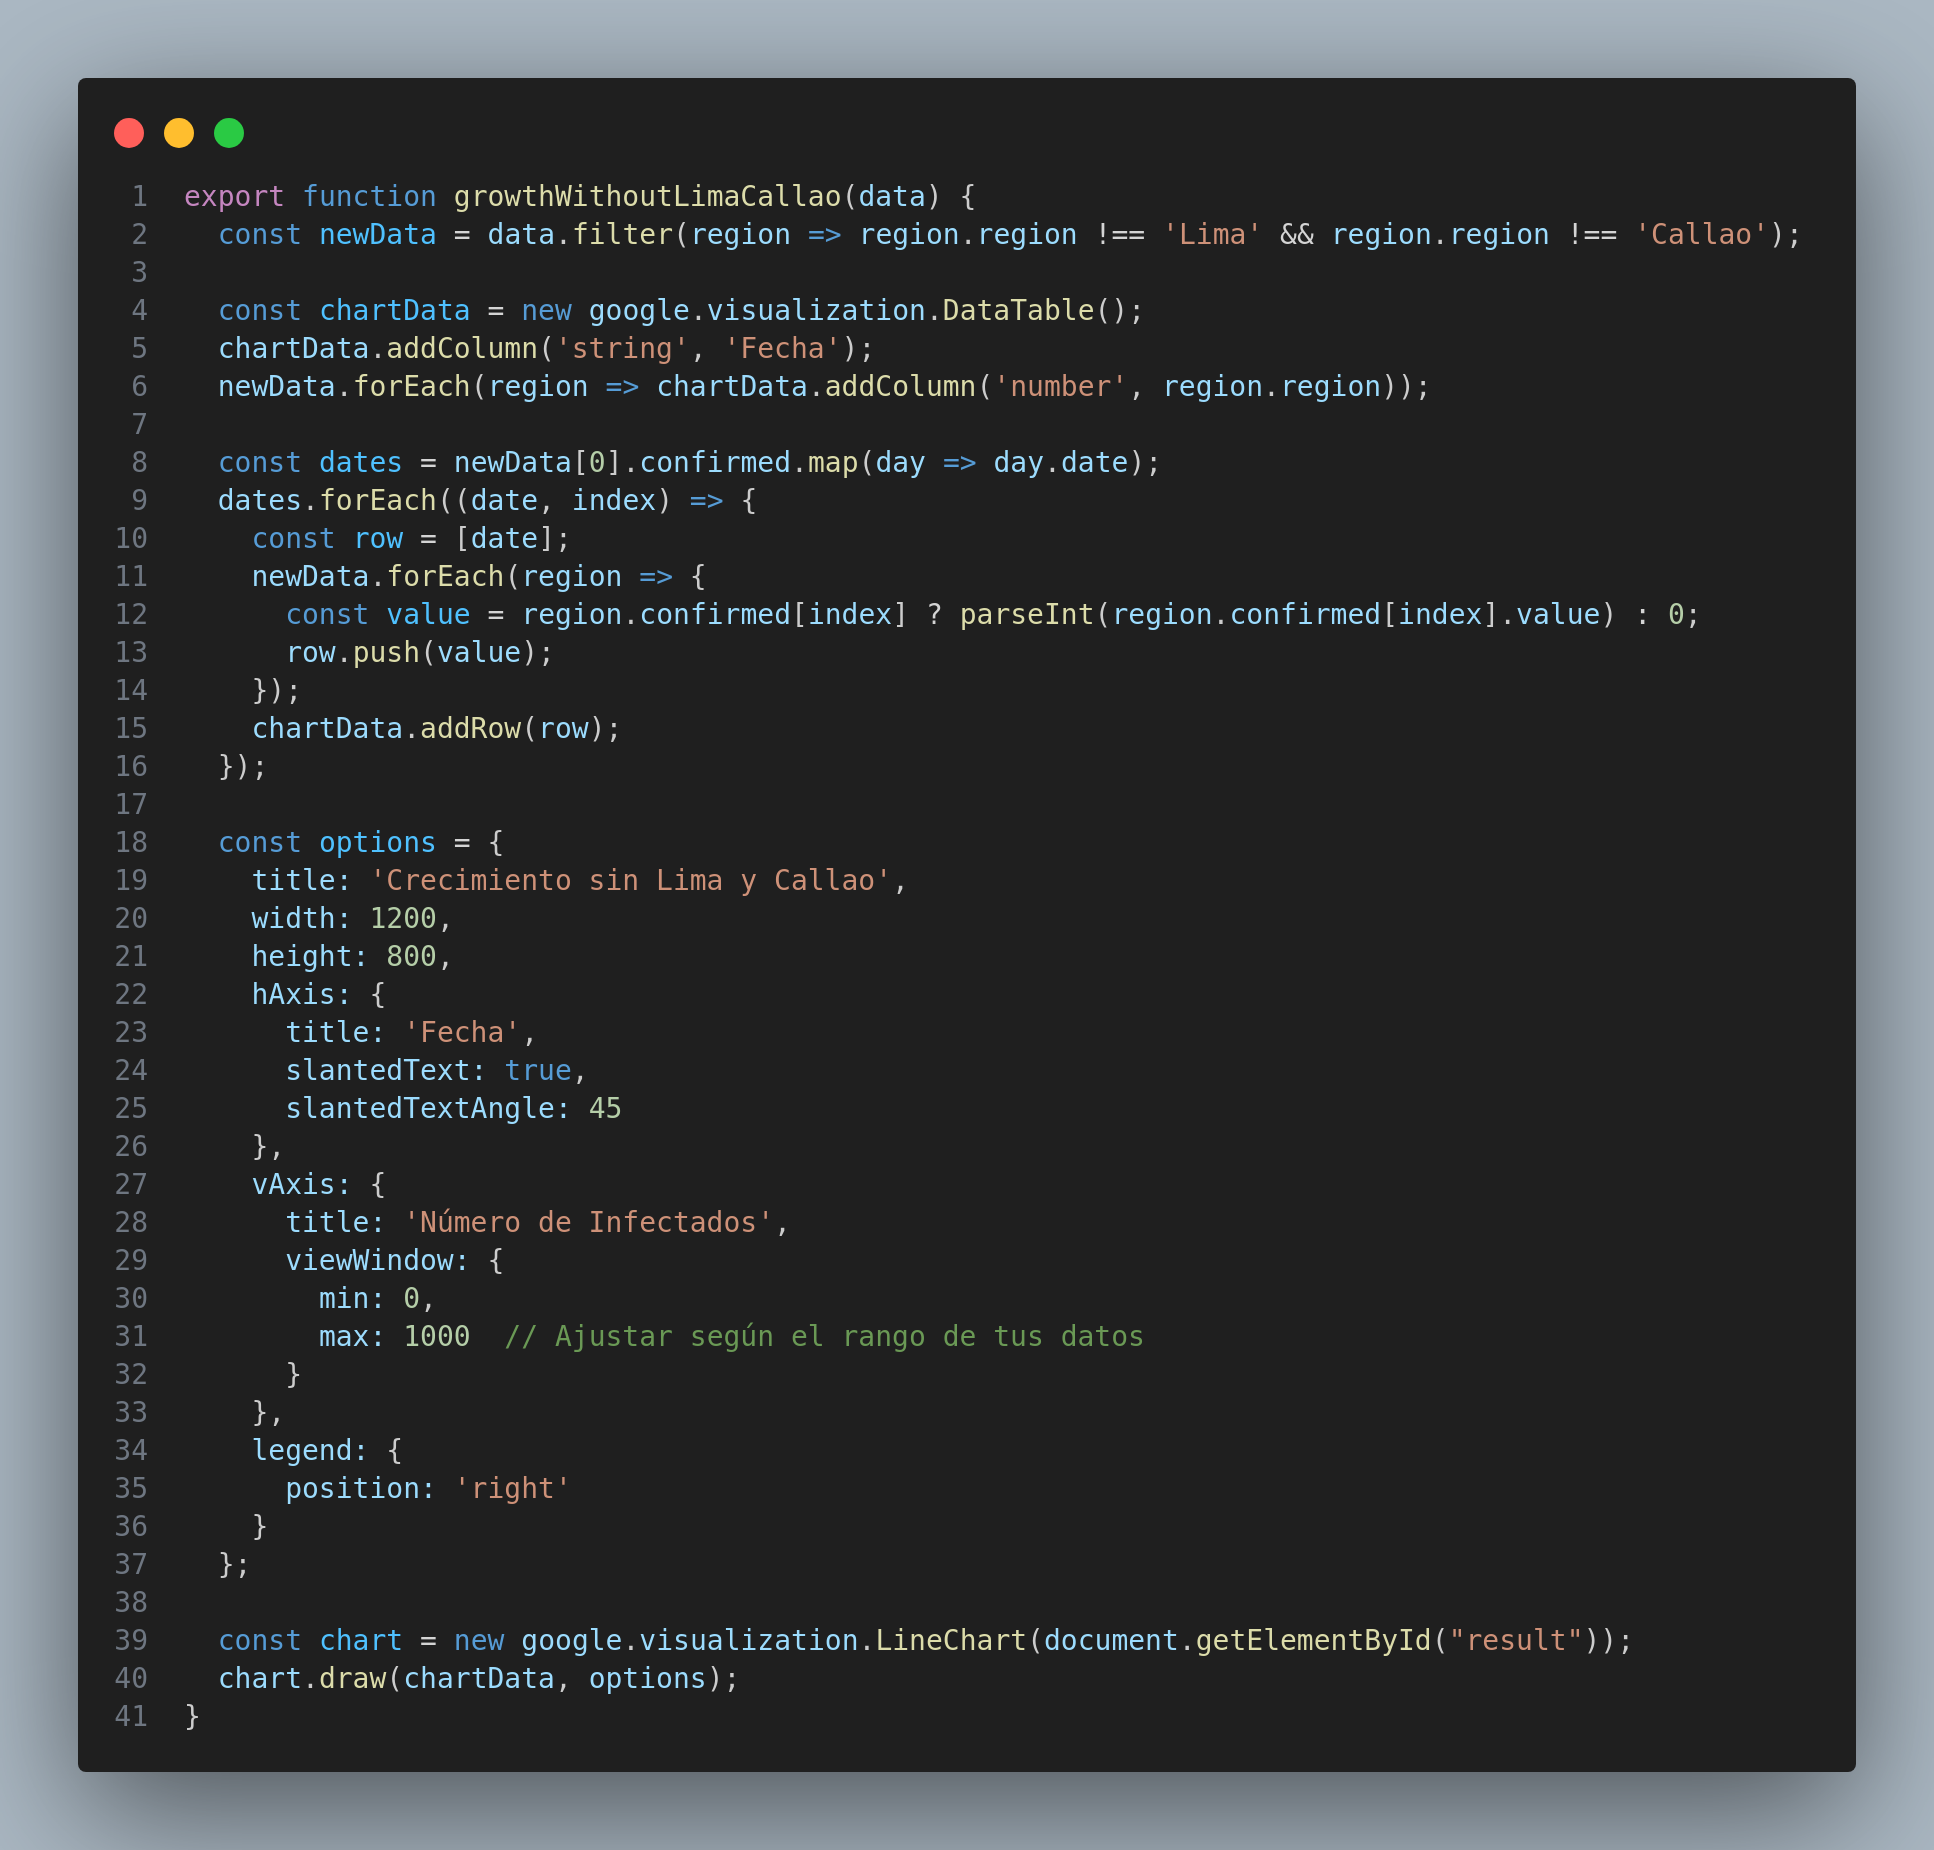
\includegraphics[width=1.0\textwidth]{img/6_js.png}
  \caption{ejercicio6.js}
\end{figure}
En el septimo ejercicio la función compareRegions compara el crecimiento de casos confirmados entre múltiples regiones utilizando una estructura similar a las funciones anteriores, pero sin excluir regiones específicas. Comienza creando una tabla de datos de Google Visualization con columnas para las fechas y cada región. Luego, añade filas de datos asumiendo que todas las regiones tienen las mismas fechas. Finalmente, genera un gráfico de líneas con opciones de configuración como título y ejes, mostrando la comparación en un elemento HTML con ID "result". Esta función simplifica el proceso de comparación al evitar la necesidad de excluir regiones específicas en el código.
\begin{figure}[H]
  \centering
  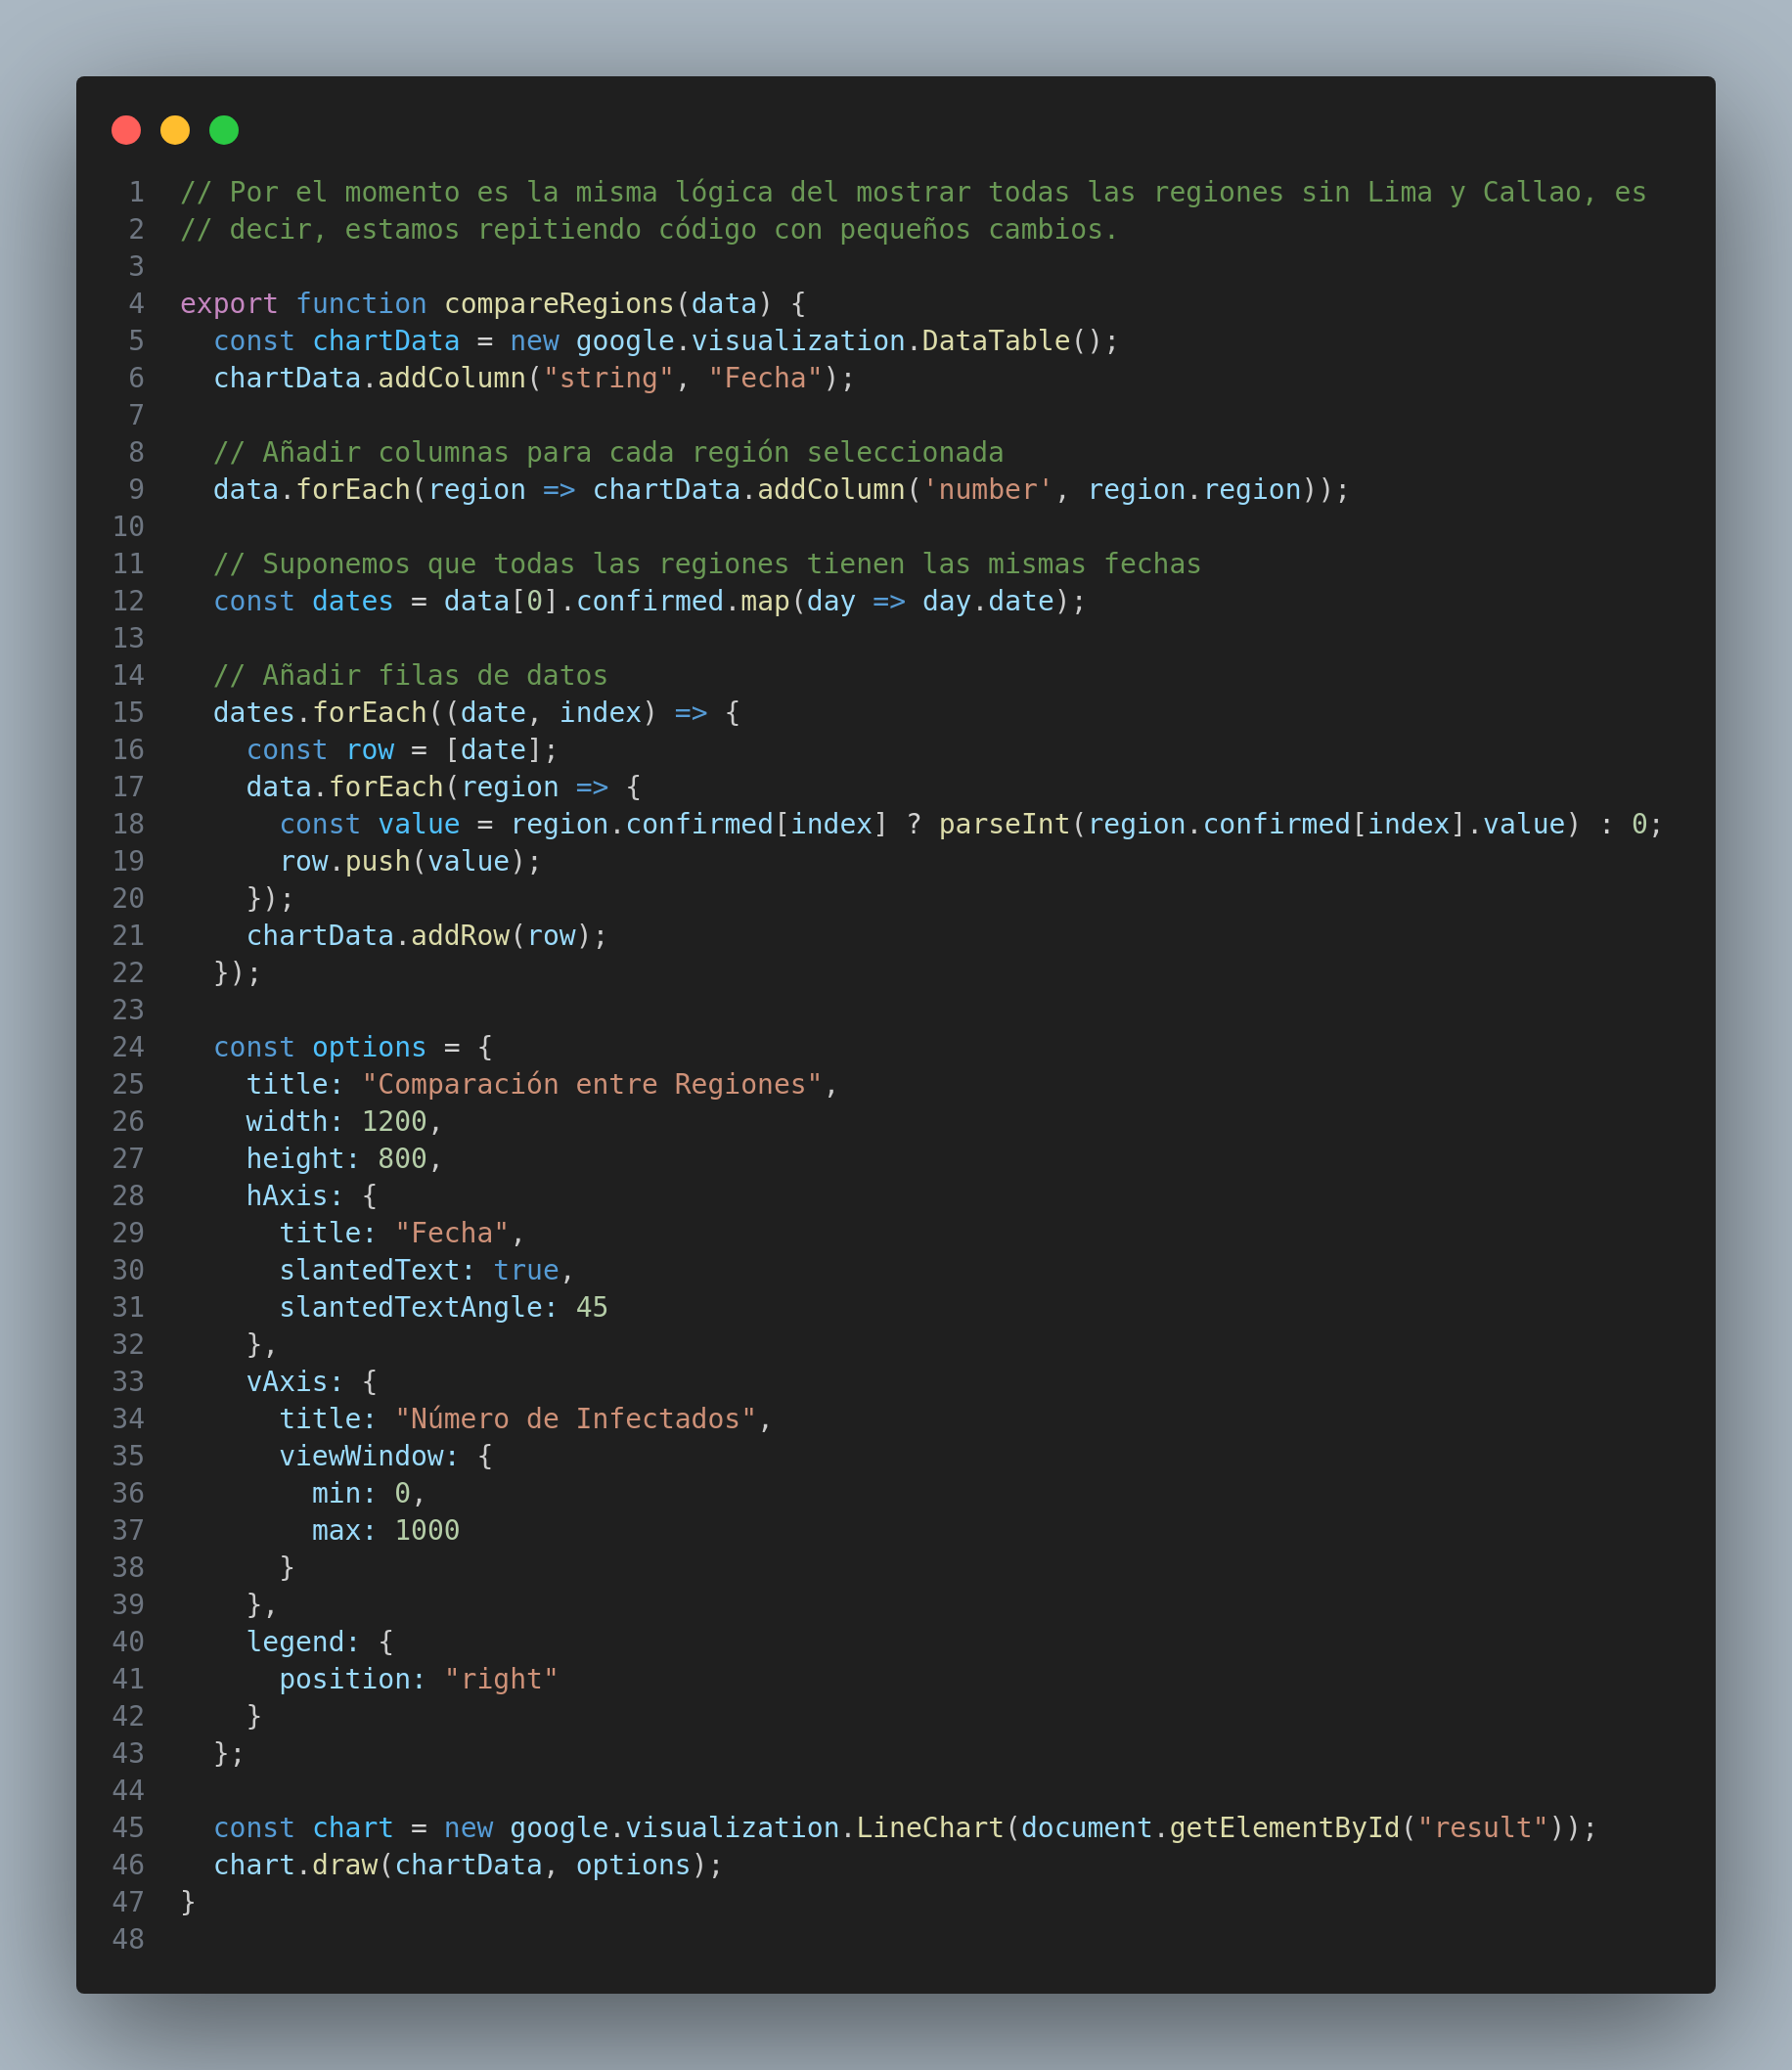
\includegraphics[width=1.0\textwidth]{img/7_js.png}
  \caption{ejercicio7.js}
\end{figure}
En el octavo ejercicio la función drawComparativeChart, genera un gráfico comparativo del crecimiento de casos de infectados en Perú, excluyendo las regiones de Lima y Callao. Filtra la información para eliminar estas dos regiones, crea una tabla de datos y prepara filas con datos de casos confirmados por fecha y región. Luego, establece opciones para el gráfico, como título y ejes, y finalmente dibuja el gráfico de líneas en un elemento HTML específico. Esta función ofrece una forma clara de comparar el avance de la enfermedad en las regiones peruanas excluyendo Lima y Callao.
\begin{figure}[H]
  \centering
  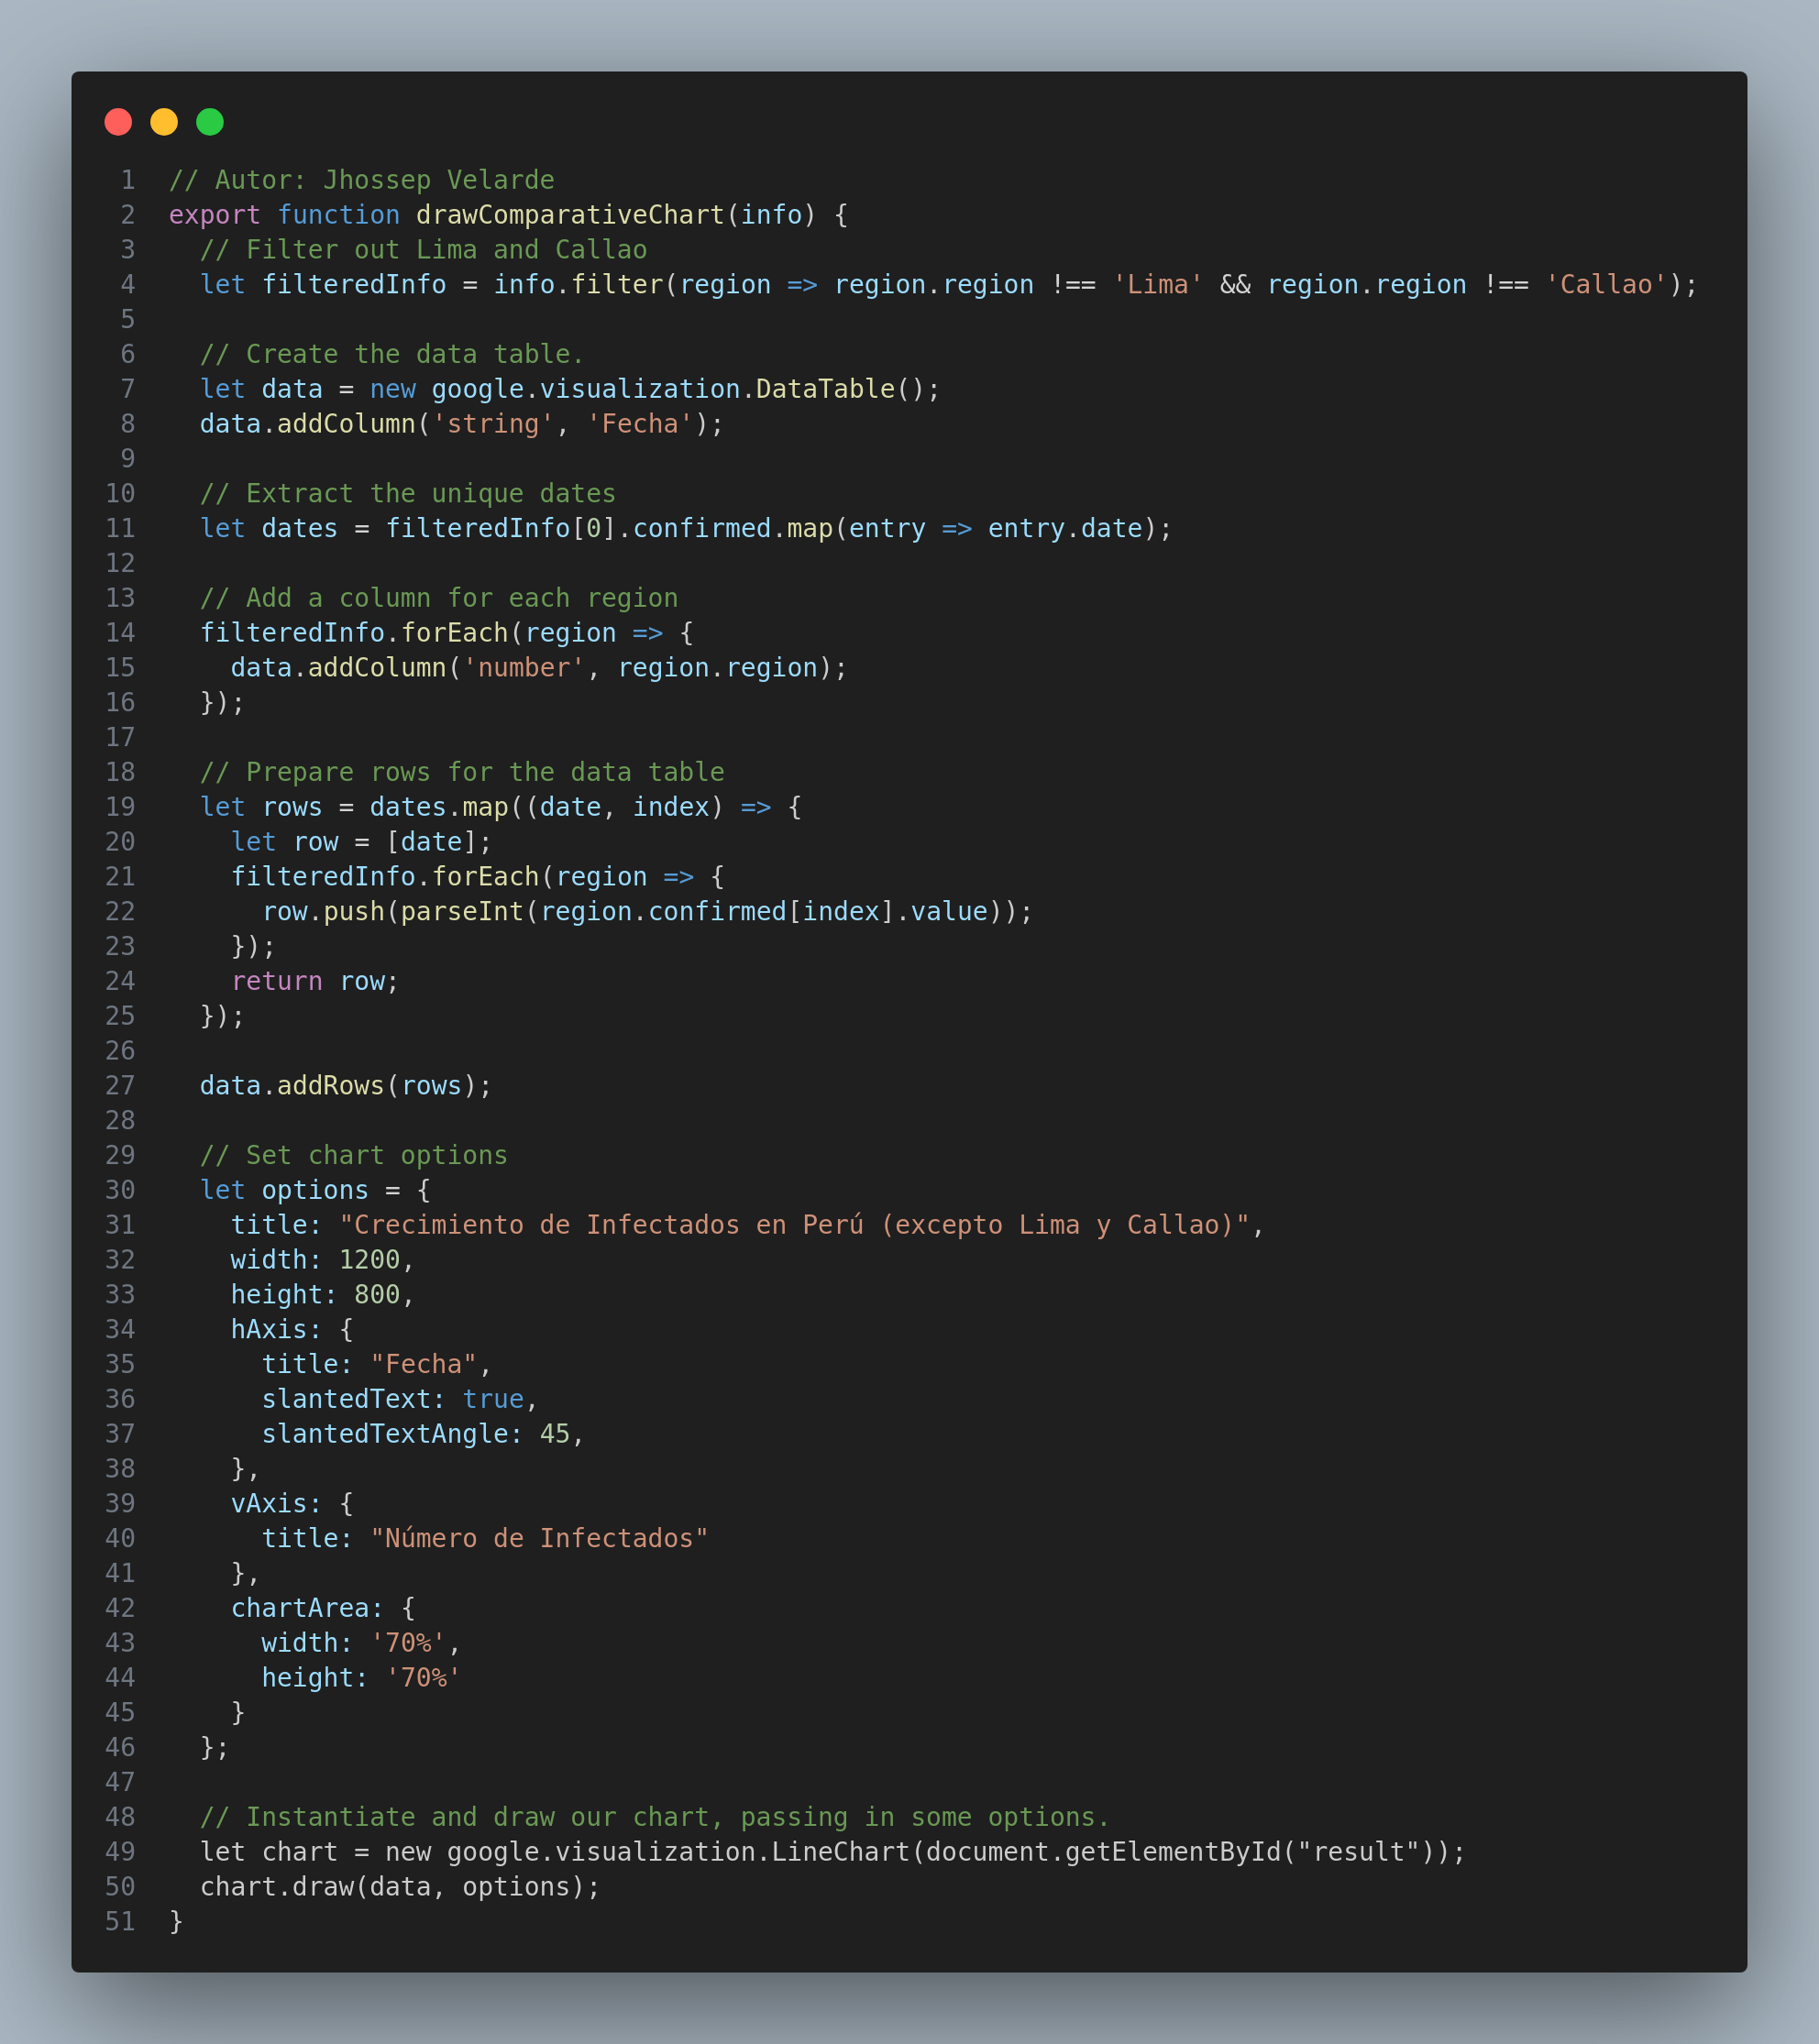
\includegraphics[width=1.0\textwidth]{img/8_js.png}
  \caption{ejercicio8.js}
\end{figure}
Tenemos un main donde se ejecutara el script importa ocho funciones desde archivos JavaScript externos, cada una diseñada para realizar una tarea específica en la visualización de datos sobre casos de infectados en regiones de Perú. Estas funciones abarcan desde la simple visualización de listas de regiones hasta la comparación detallada del crecimiento de casos confirmados en diferentes áreas geográficas. Al asociar cada función a un botón en la interfaz de usuario, el script permite una fácil interacción del usuario, lo que facilita la exploración y comprensión de los datos sobre la situación de la pandemia en Perú.
\begin{figure}[H]
  \centering
  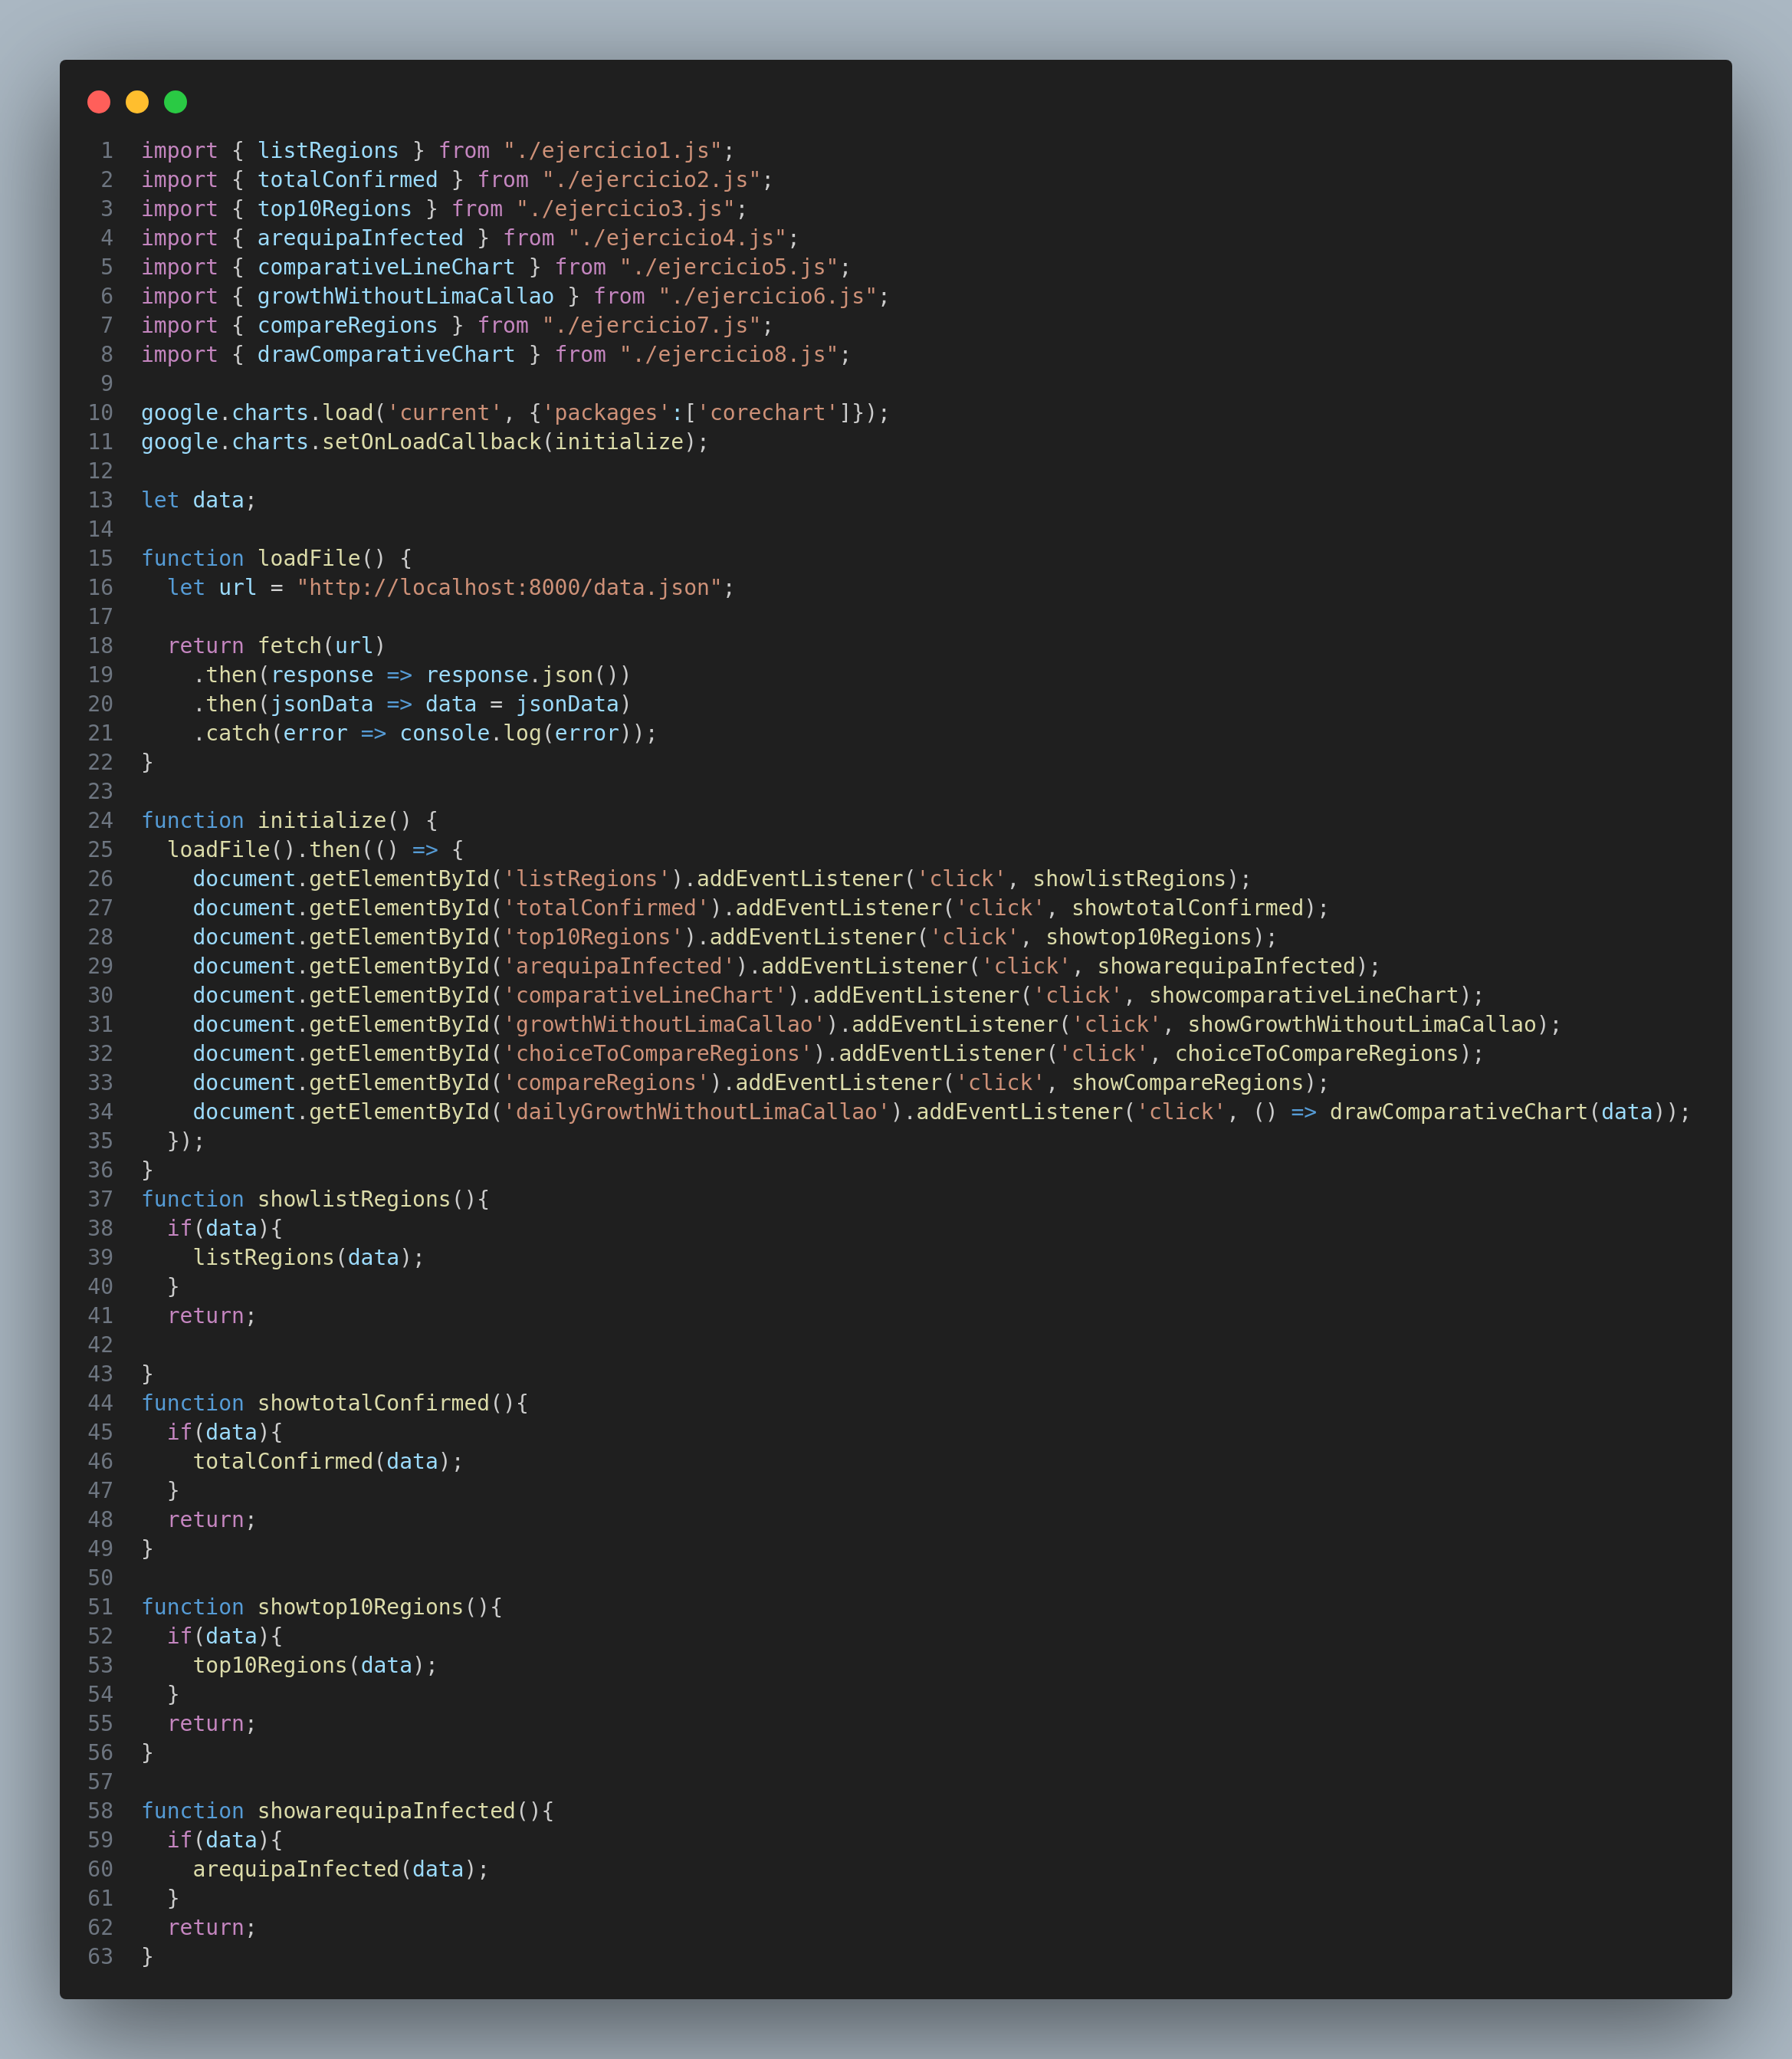
\includegraphics[width=1.0\textwidth]{img/main1_js.png}
  \caption{main.js}
\end{figure}
\begin{figure}[H]
  \centering
  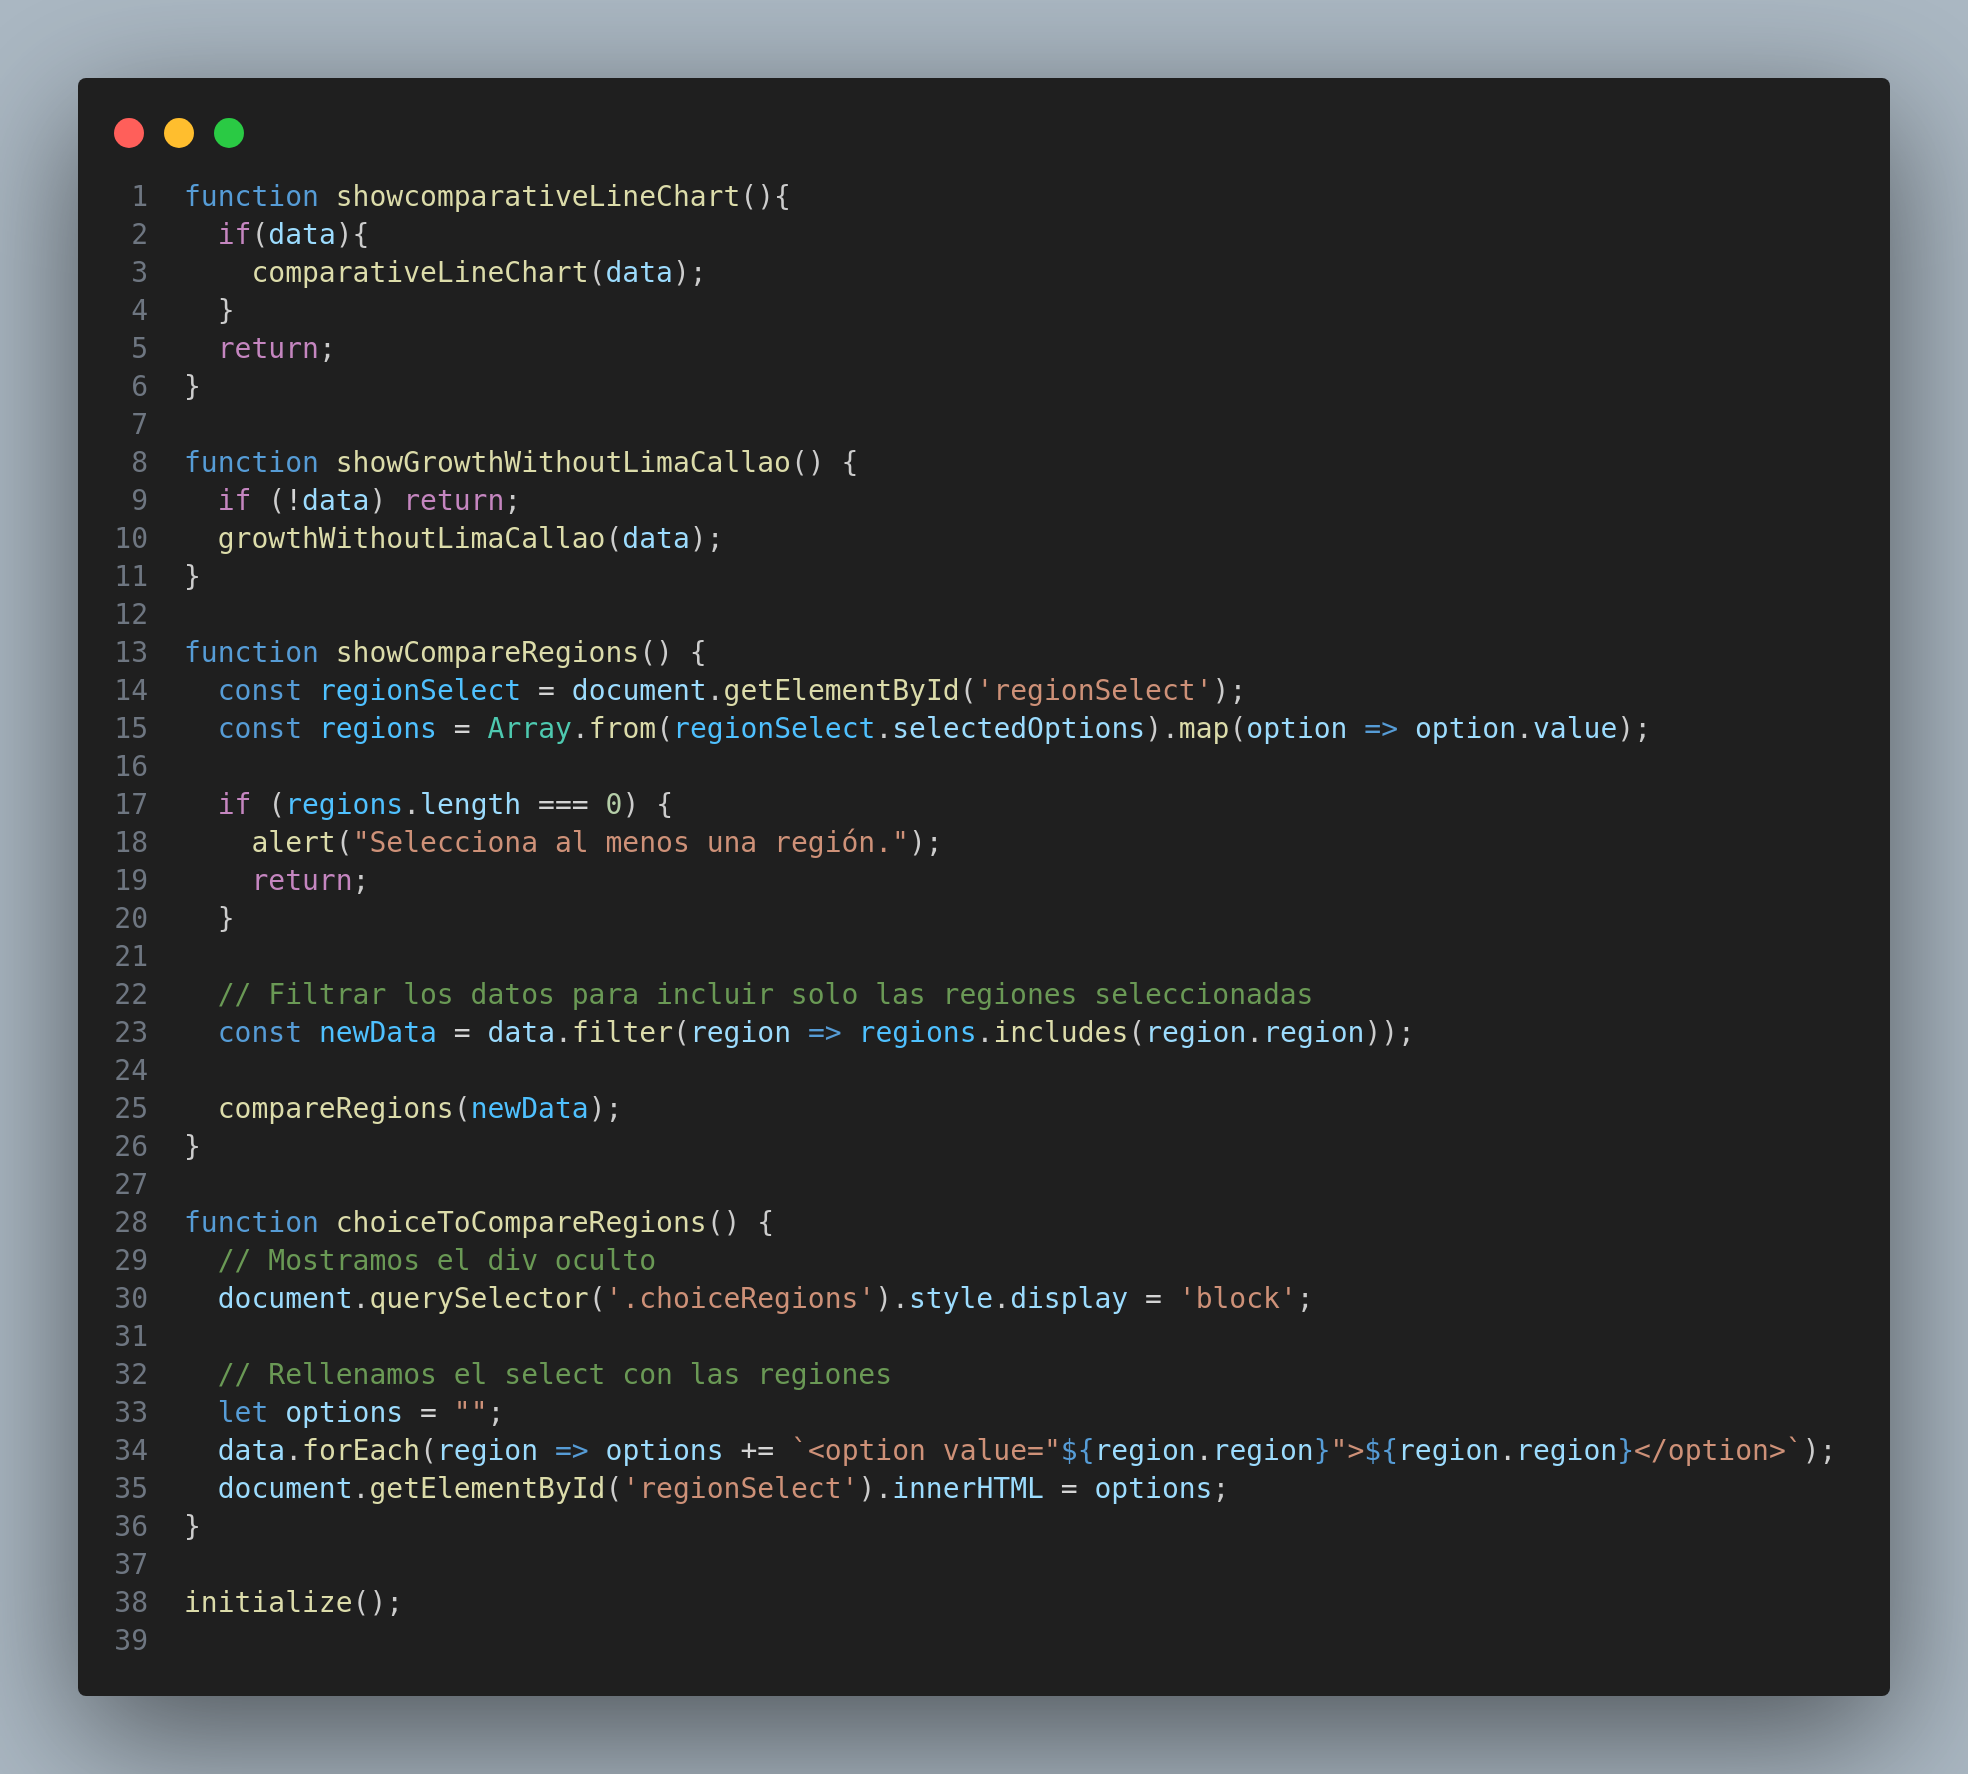
\includegraphics[width=1.0\textwidth]{img/main2_js.png}
  \caption{main.js}
\end{figure}

\section{La ejecucion de los 8 ejercicios en el index.HTML}
El primero :
\begin{figure}[H]
  \centering
  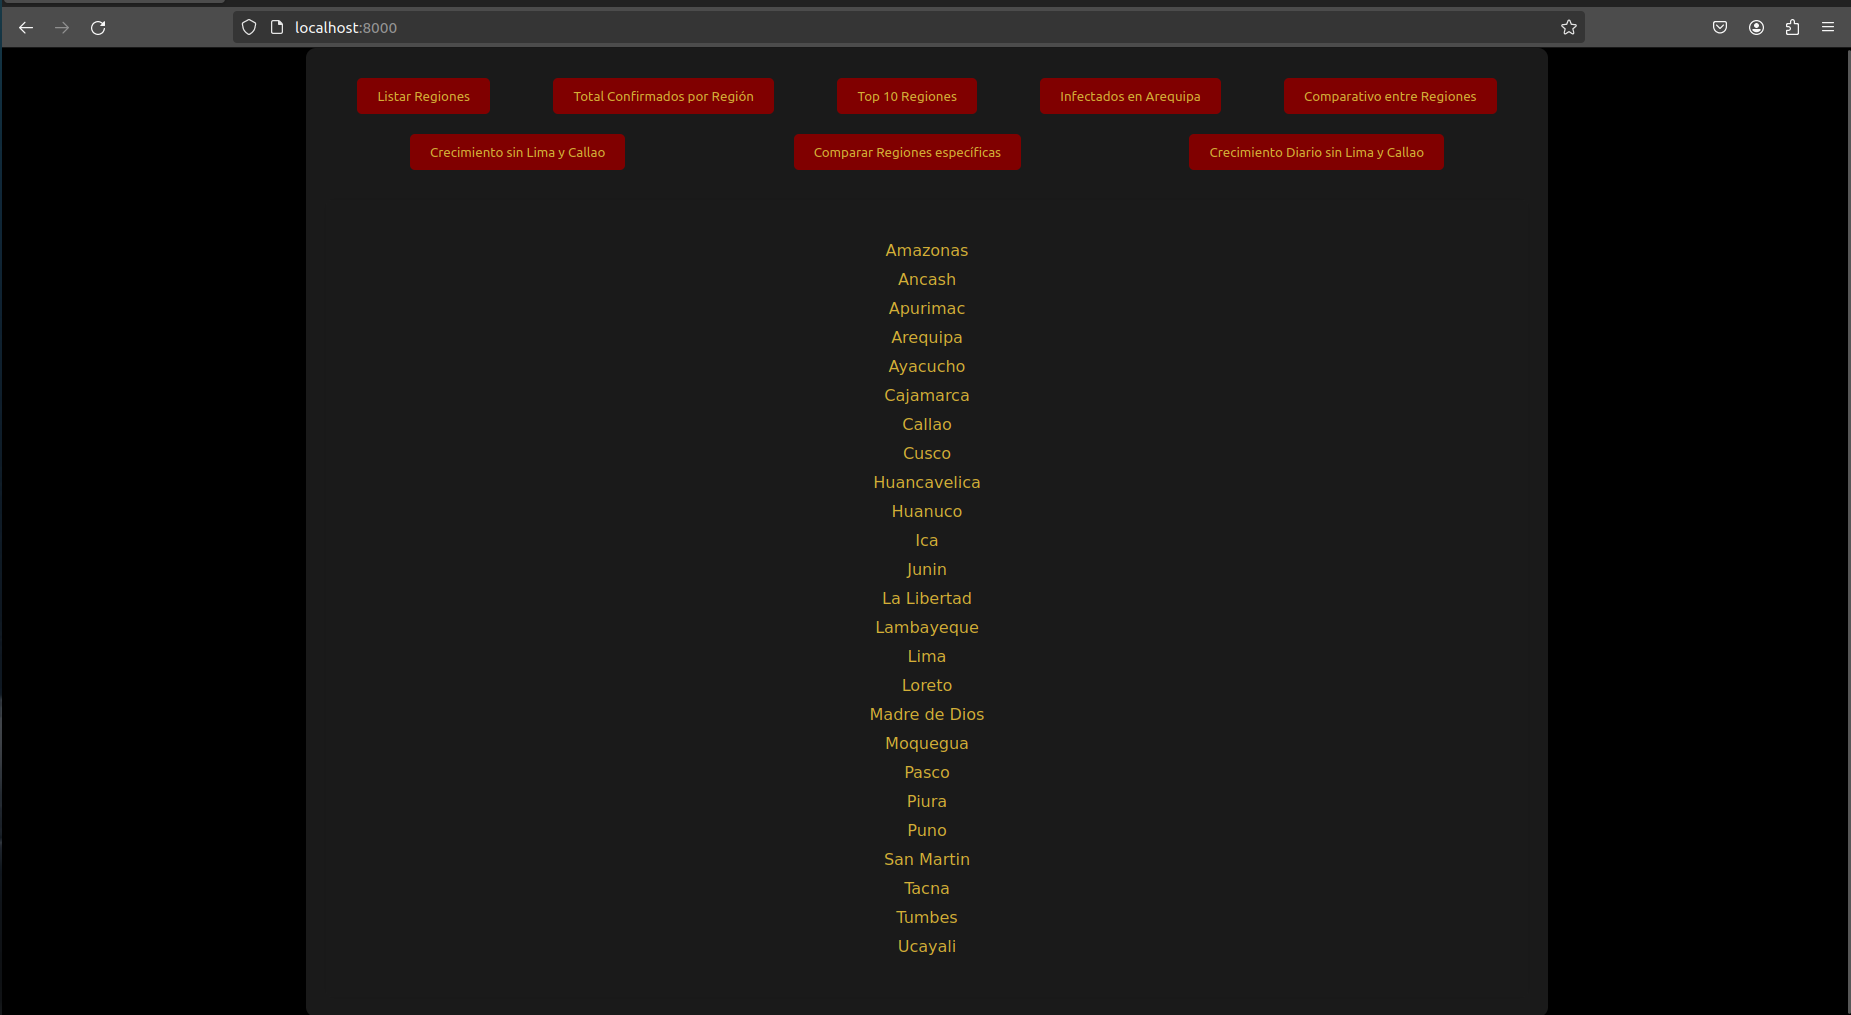
\includegraphics[width=1.0\textwidth]{img/Ej1.png}
  \caption{Ejecucion}
\end{figure}
El segundo :
\begin{figure}[H]
  \centering
  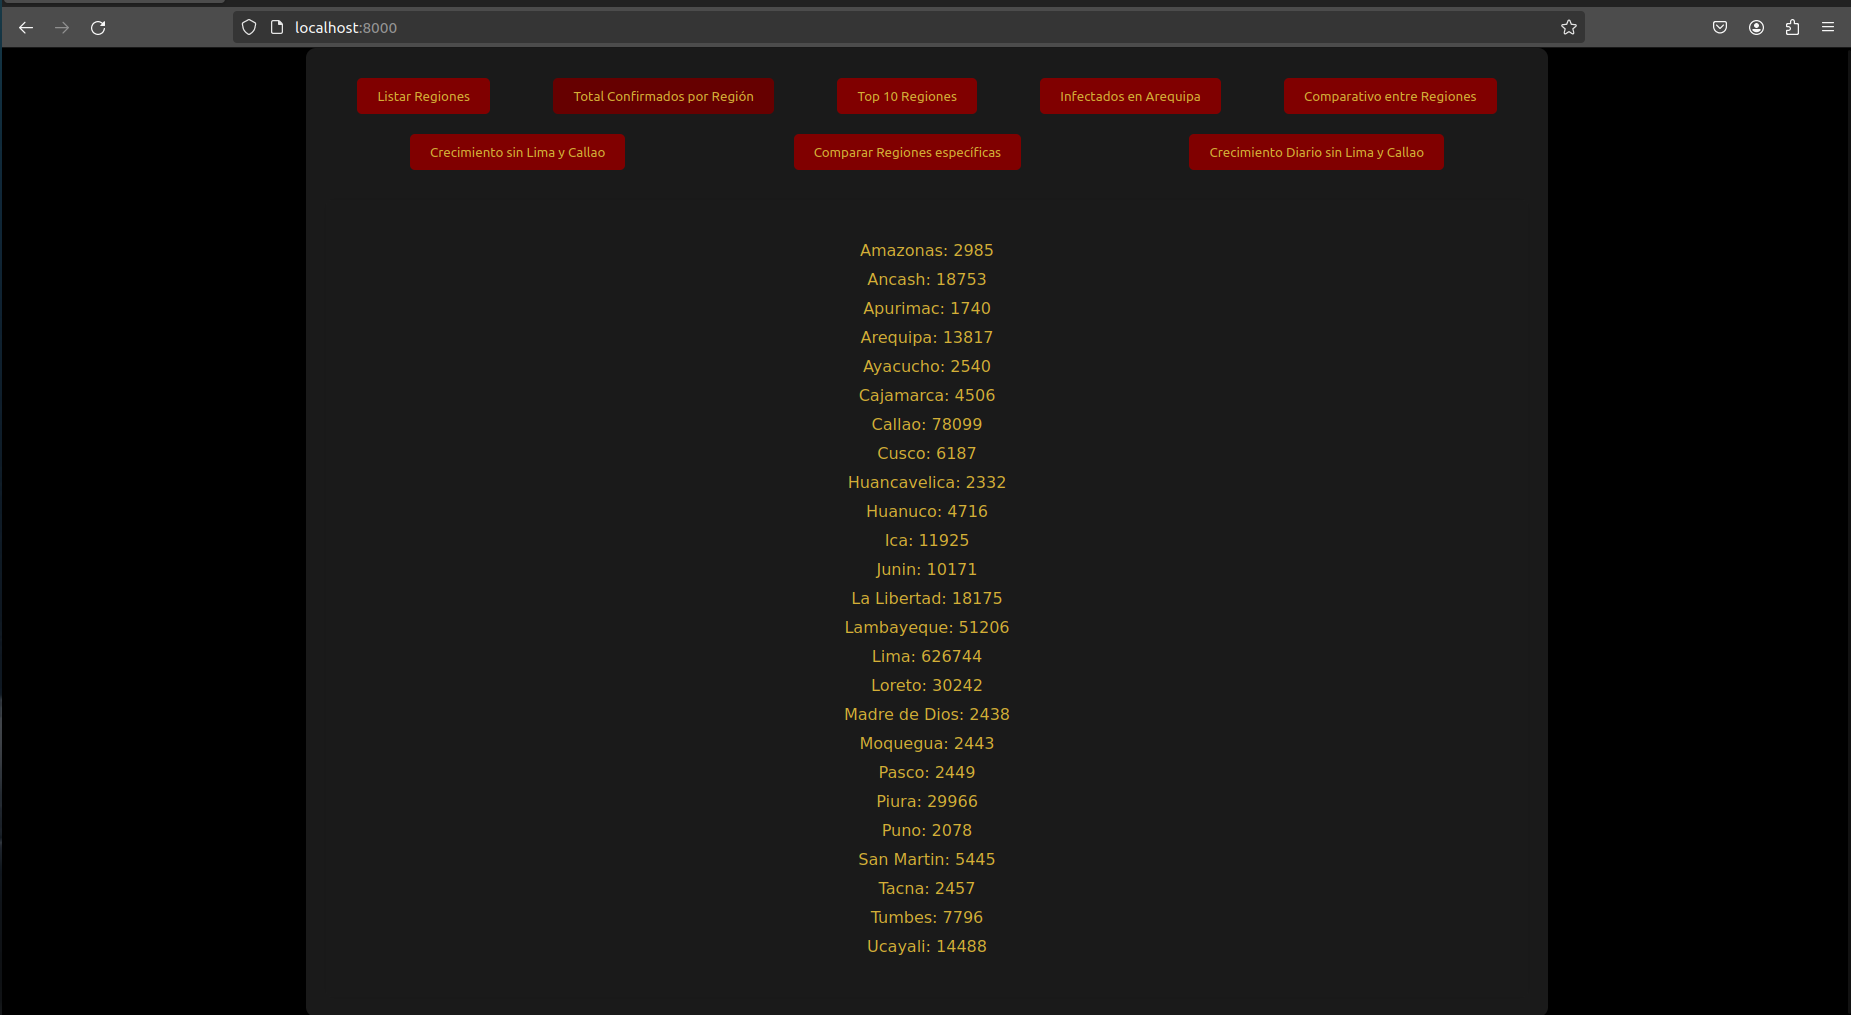
\includegraphics[width=1.0\textwidth]{img/Ej2.png}
  \caption{Ejecucion}
\end{figure}
El tercero :
\begin{figure}[H]
  \centering
  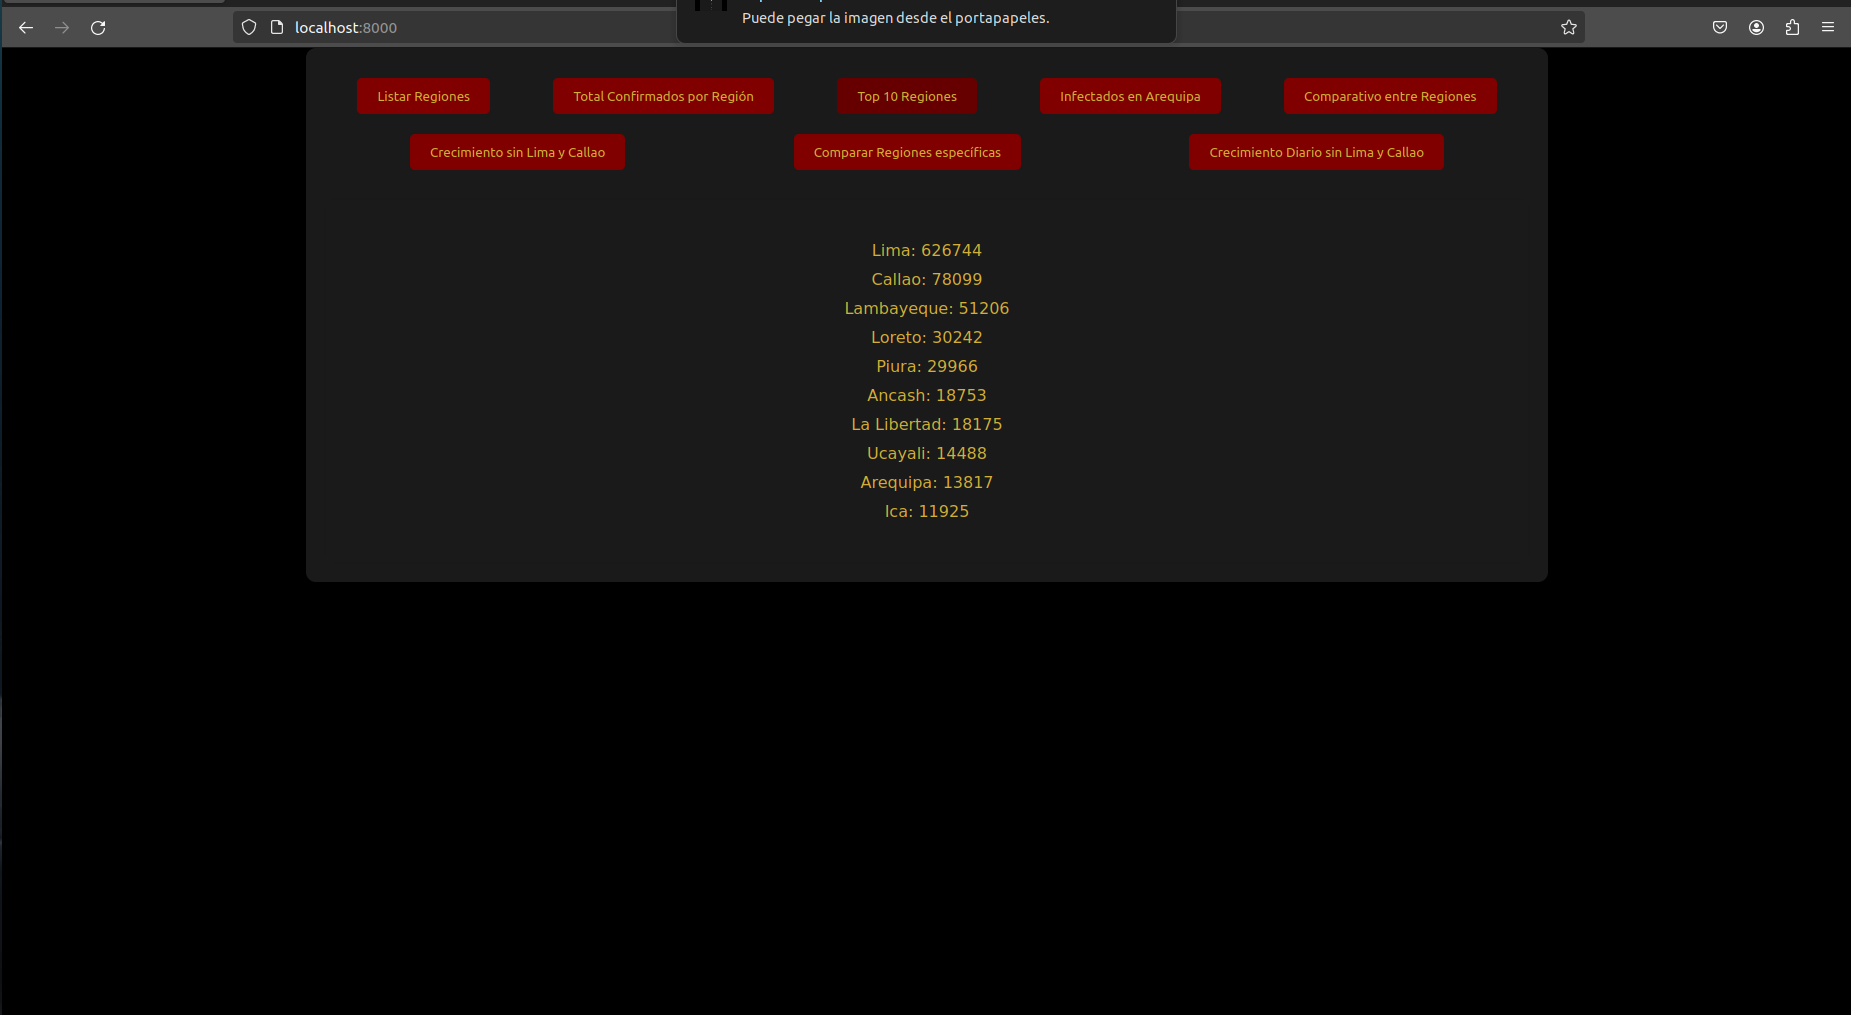
\includegraphics[width=1.0\textwidth]{img/Ej3.png}
  \caption{Ejecucion}
\end{figure}
El cuarto :
\begin{figure}[H]
  \centering
  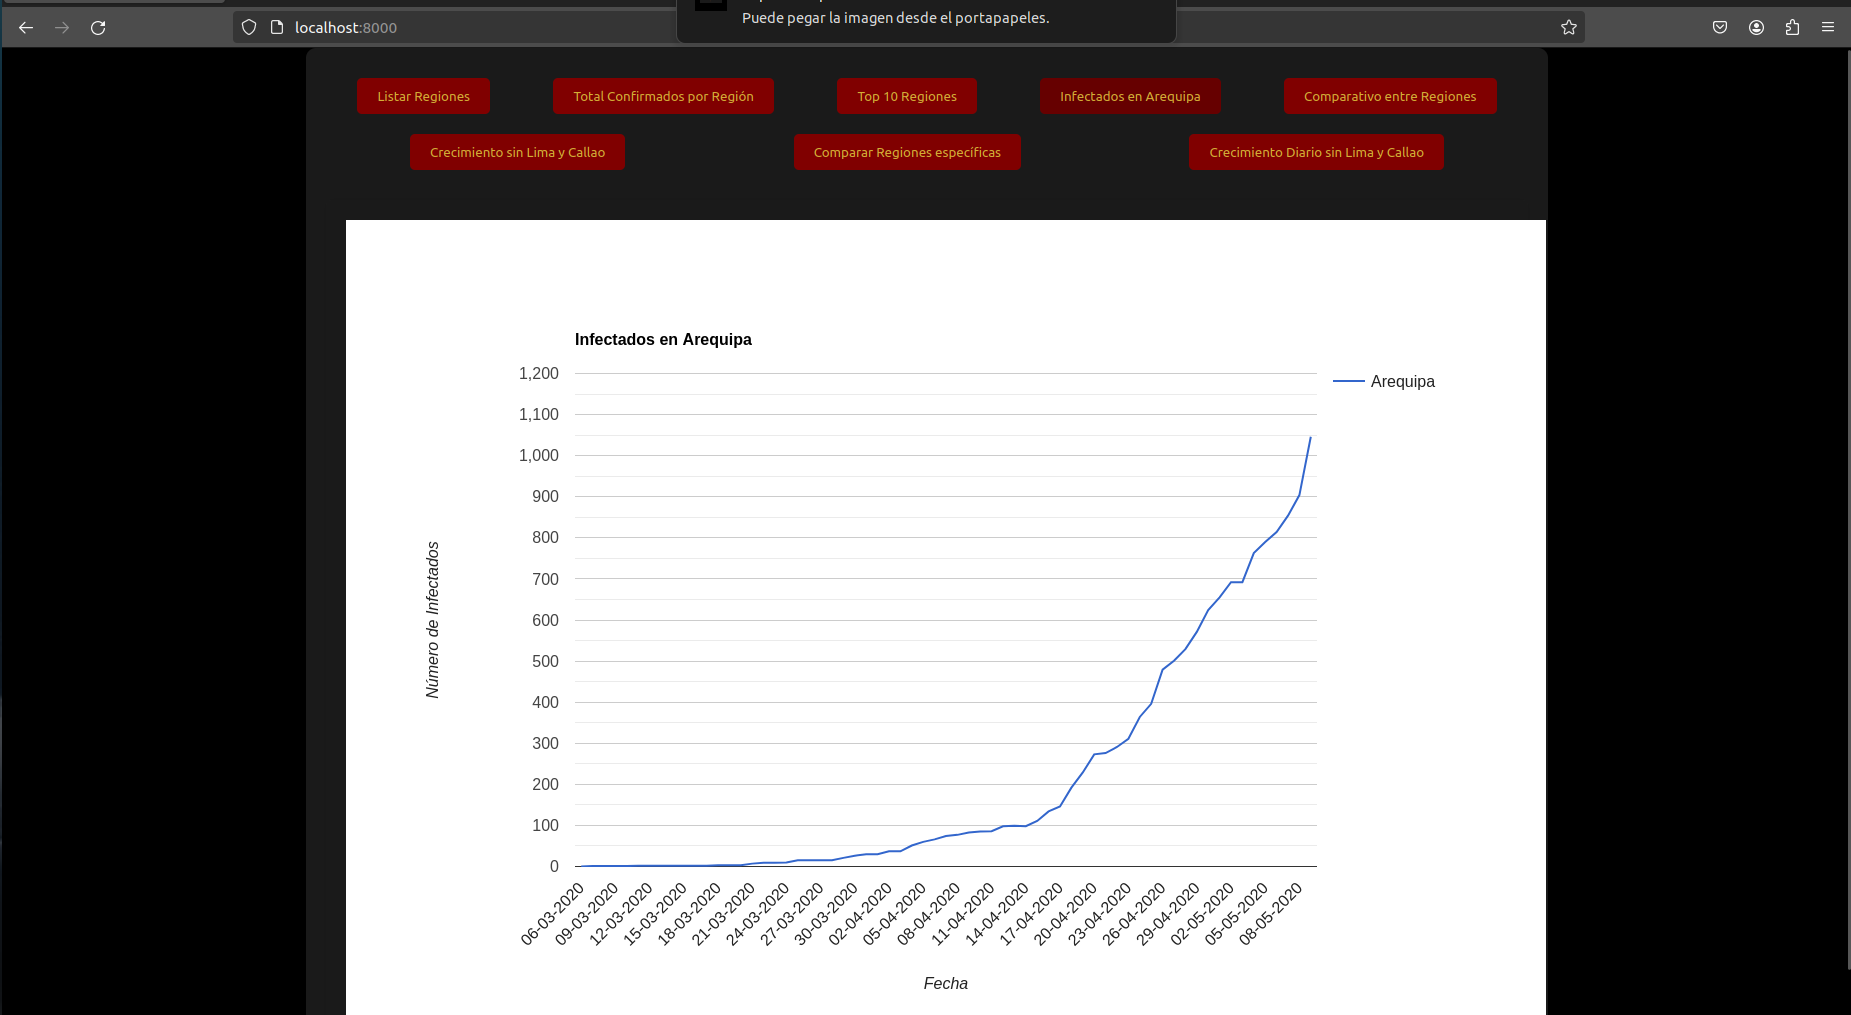
\includegraphics[width=1.0\textwidth]{img/Ej4.png}
  \caption{Ejecucion}
\end{figure}
El quinto :
\begin{figure}[H]
  \centering
  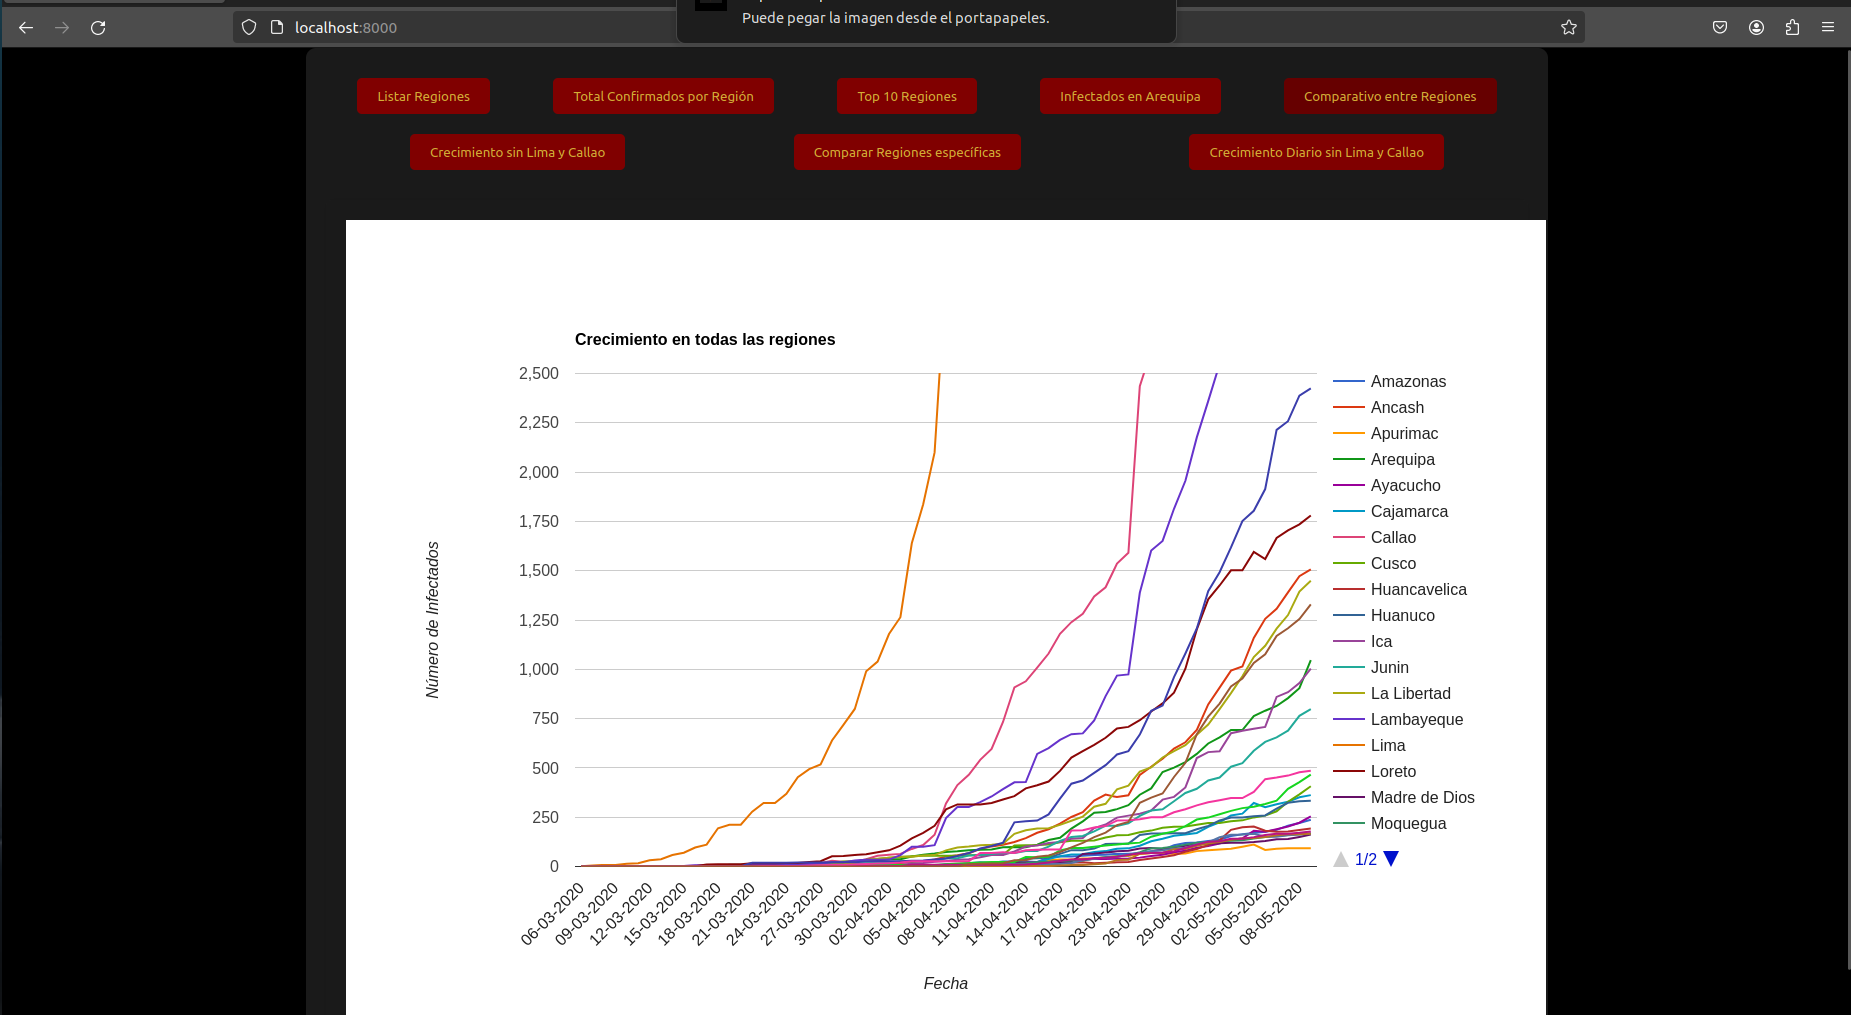
\includegraphics[width=1.0\textwidth]{img/Ej5.png}
  \caption{Ejecucion}
\end{figure}
El sexto :
\begin{figure}[H]
  \centering
  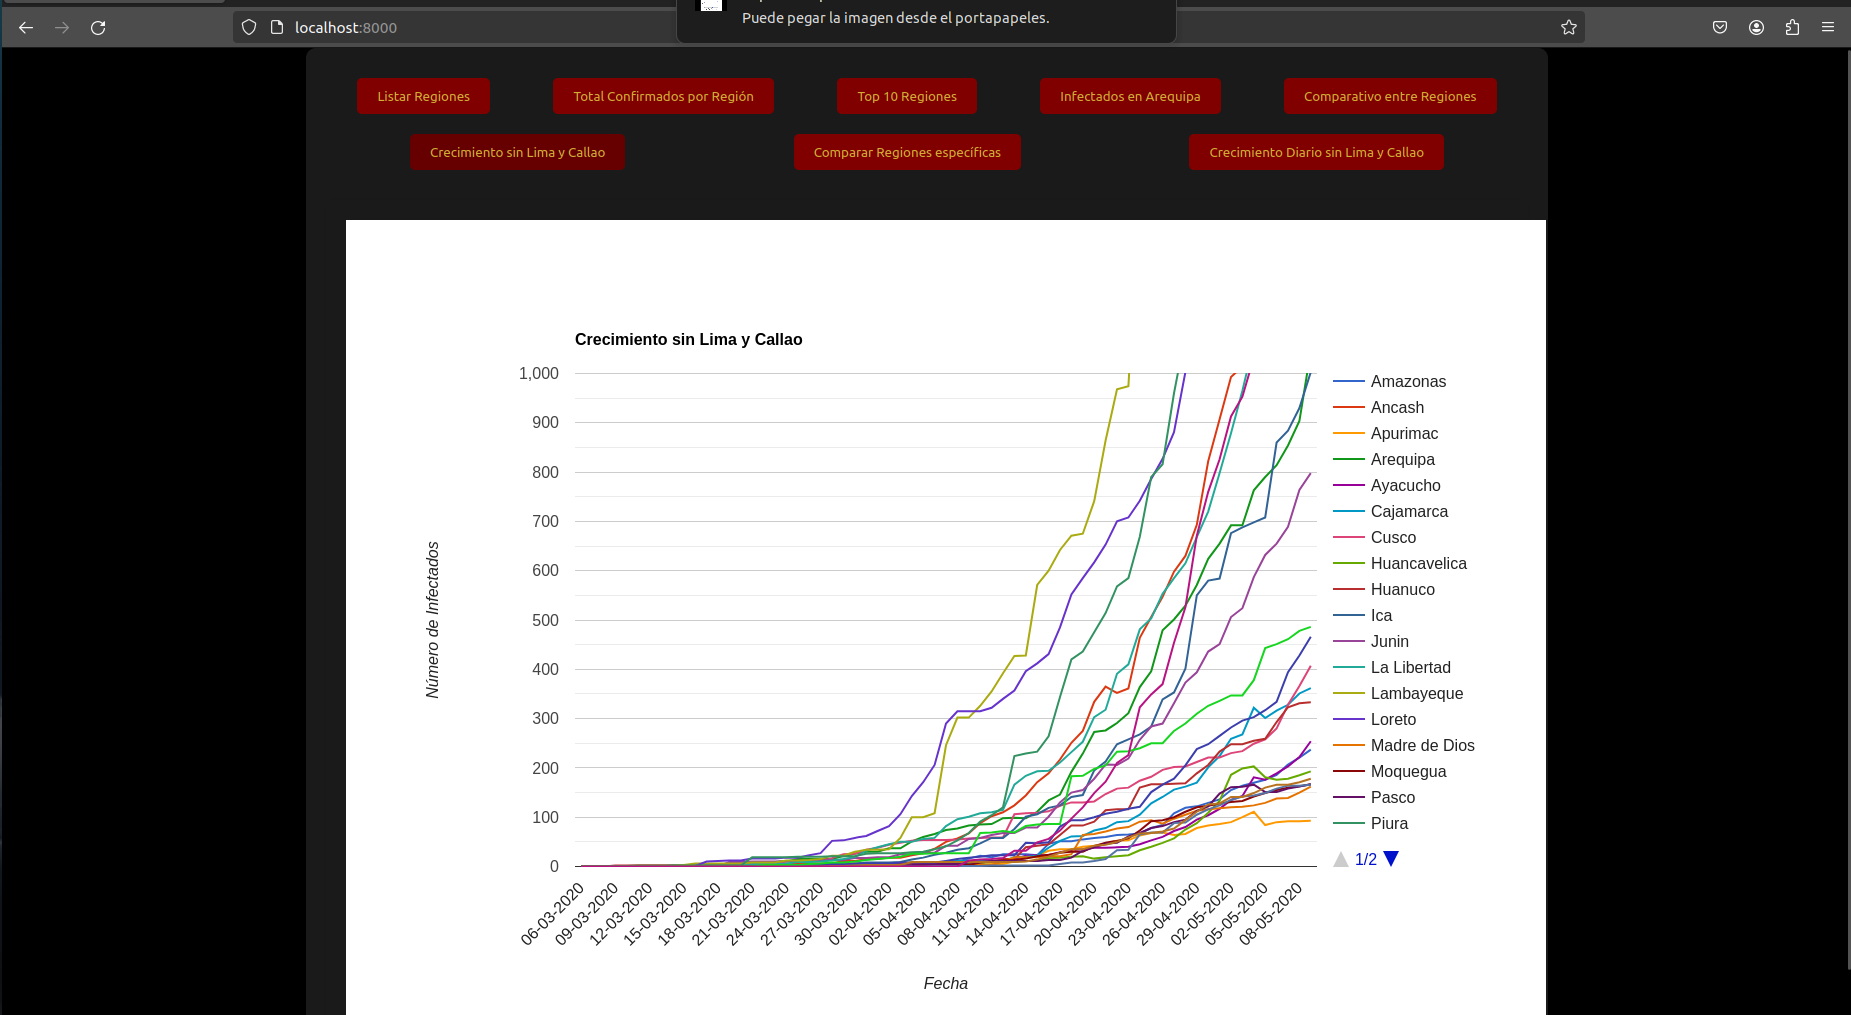
\includegraphics[width=1.0\textwidth]{img/Ej6.png}
  \caption{Ejecucion}
\end{figure}
El septimo :
\begin{figure}[H]
  \centering
  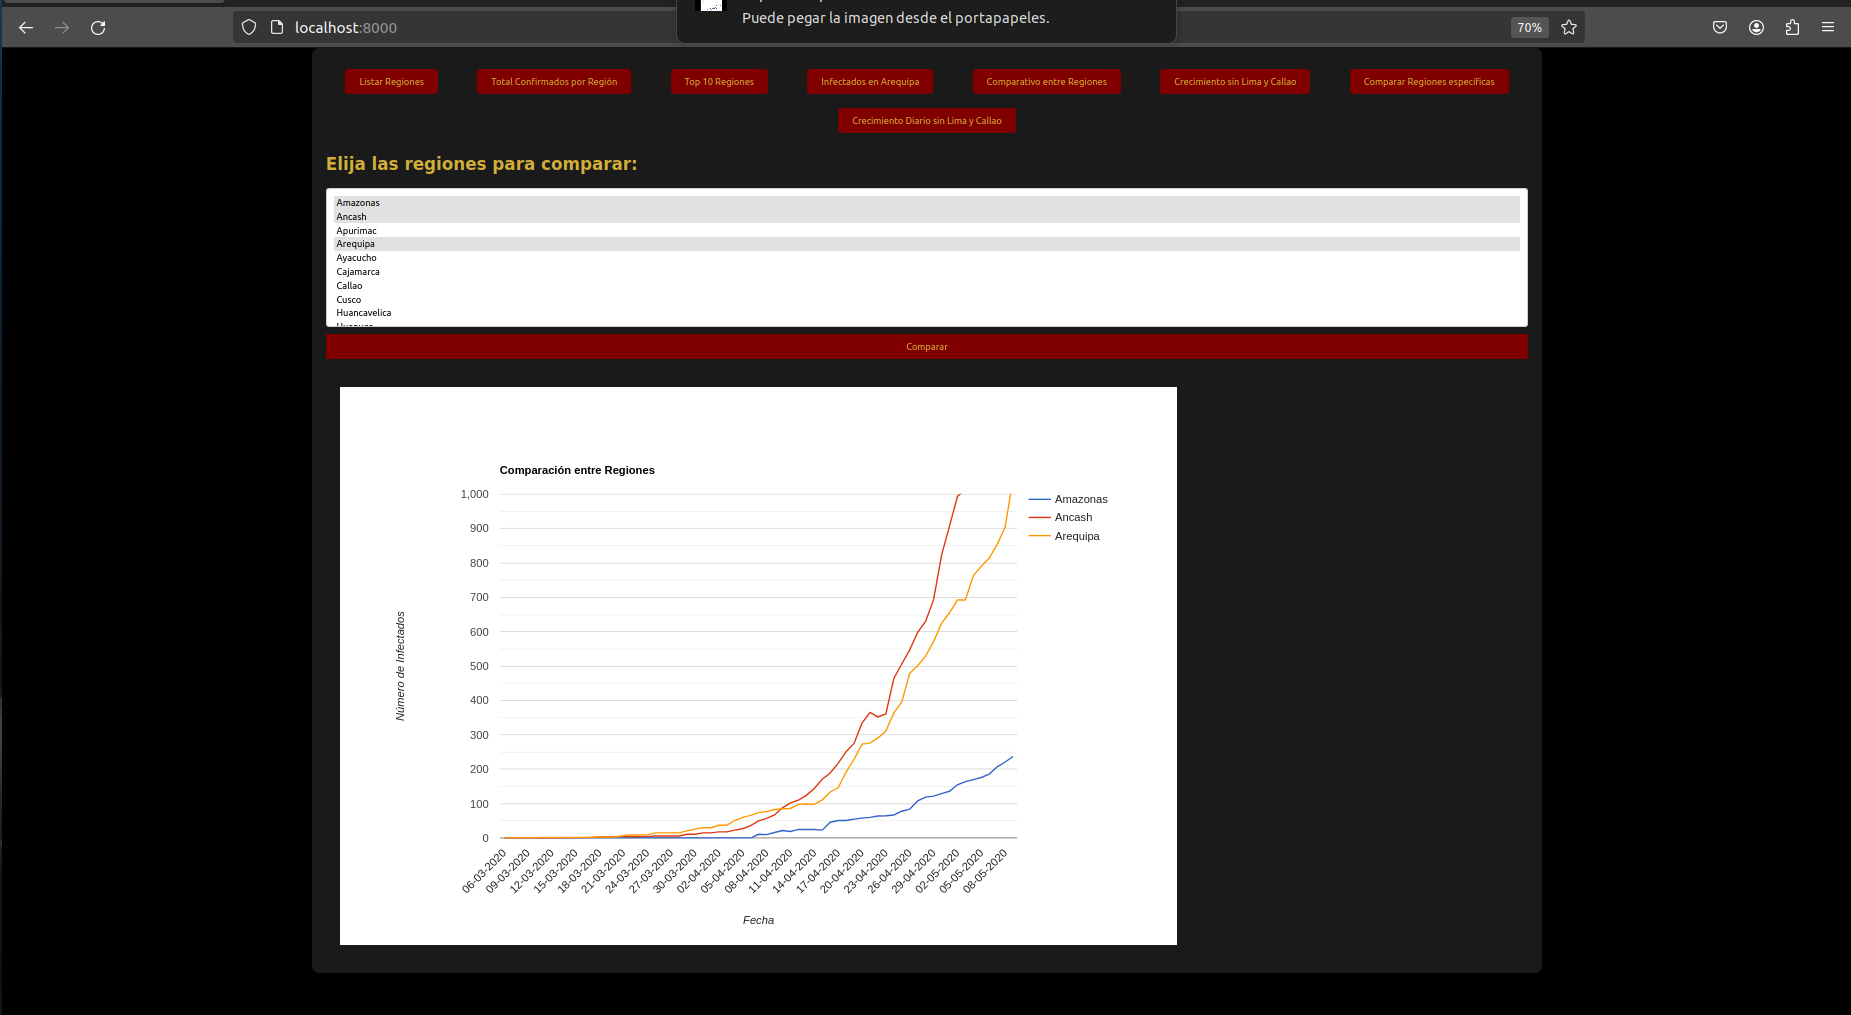
\includegraphics[width=1.0\textwidth]{img/Ej7.png}
  \caption{Ejecucion}
\end{figure}
El octavo :
\begin{figure}[H]
  \centering
  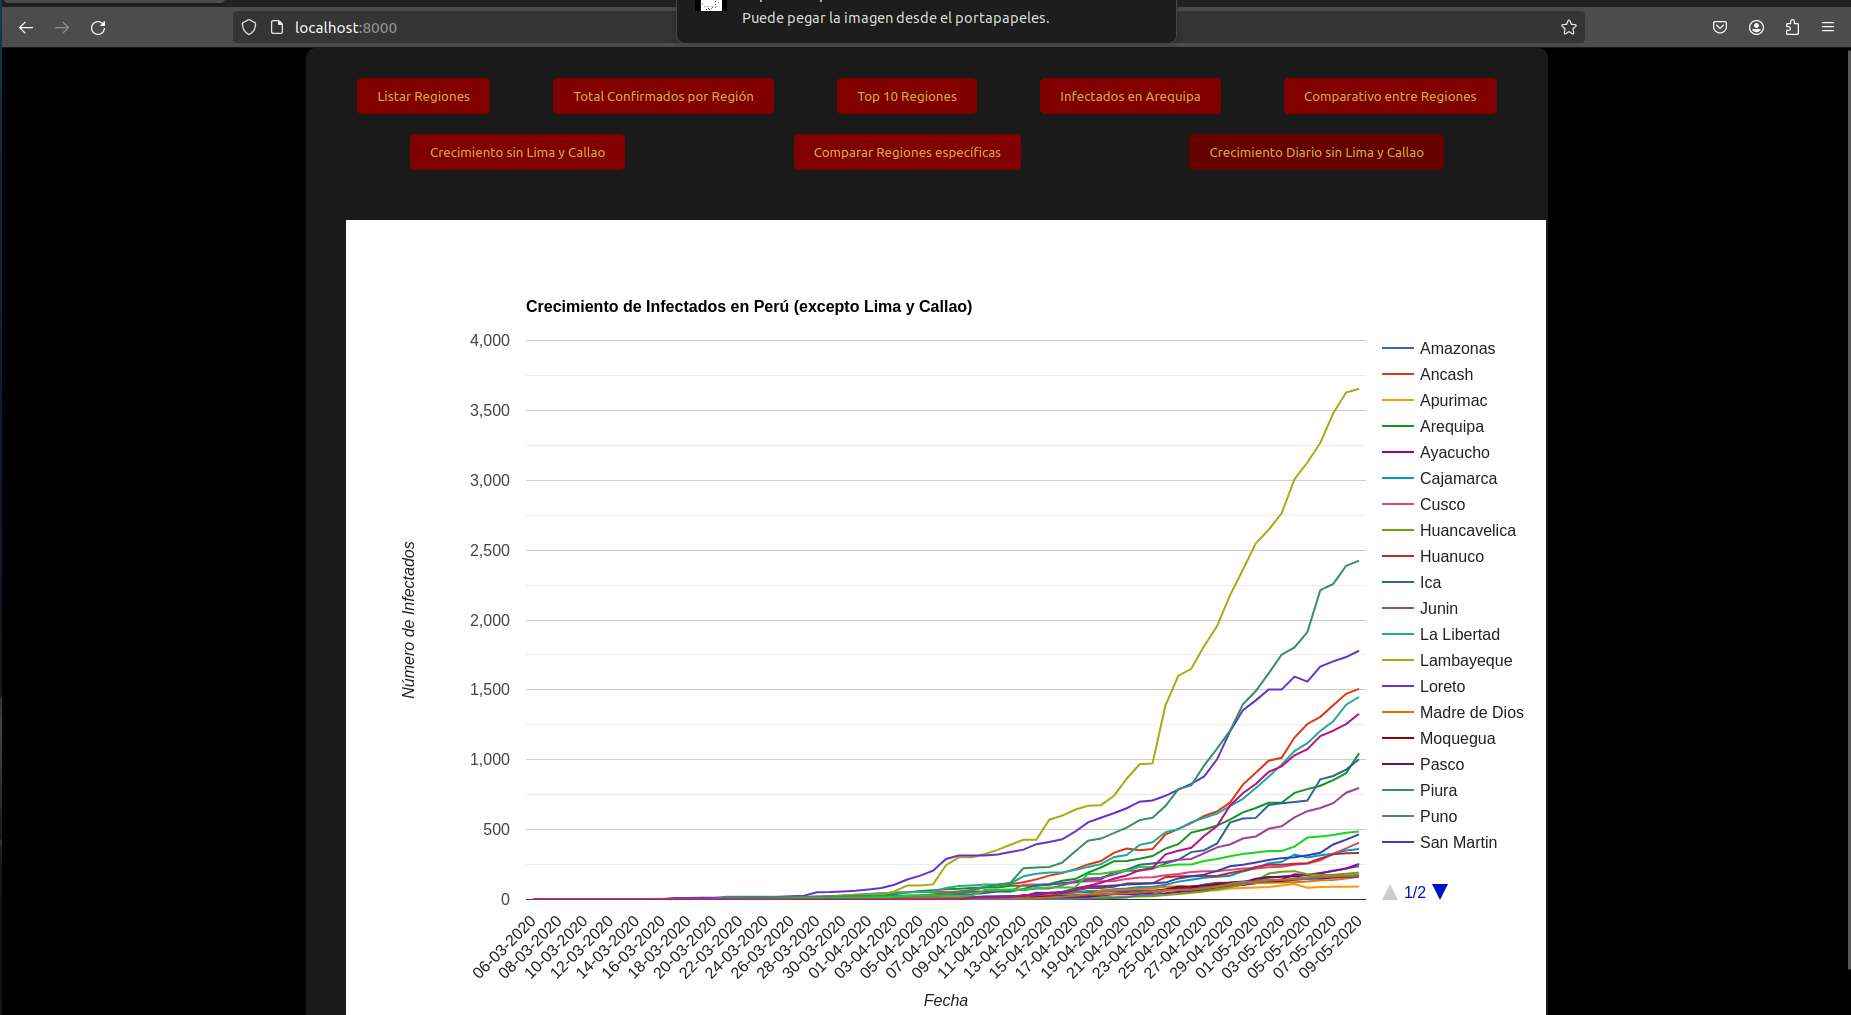
\includegraphics[width=1.0\textwidth]{img/Ej8.png}
  \caption{Ejecucion}
\end{figure}